\chapter{Related Work}


In diesem Kapitel werden die Grundlagen für die folgenden Kapitel gelegt und der Zusammenhänge hergestellt. Im ersten Teil wird zuerst ein Überblick über die Architektur eines Datenbanksystems vor dem Hintergrund der Anfragenoptimierung gegeben. Der für die Optimierung wichtige Begriff des Search Spaces erläutert. In ihm können mit Hilfe von Enumeratoren alternative, äquivalente Pläne gefunden werden und aus diesen Plänen durch eine Kostenschätzung der optimale Plan gefunden werden. Auch die Techniken der Enumeration und Kostenschätzung werden in ihrer Funktion beschrieben.

Neben diesen Grundbegriffen werden auch konkrete Implementierungen von Datenbanksystemen und deren Anfragenoptimierern besprochen. Neben System R, das die Grundlage für alle weiteren Anfragenoptimierer bildet, wird auch IBMs Starburst Projekt, die Projekte rund um Vulcano und Oracles DBMS besprochen und deren Unterschiede aufgezeigt.

Im nächsten Schritt wird auf die konkrete Implementierung der Suche nach alternativen Plänen am Beispiel von Volcano und dessen regelbasierten Anfragenoptimierer. Die Regelsets von \cite{pellenkoft1997complexity}, \cite{pellenkoft1997duplicate} werden abgegbildet.

Nachdem der Aufbau von DBMSen, Anfrageoptimierern und konkrete Beispiele bekannt sind, wird auf die Arbeit von \cite{shanbhag2014optimizing} eingegangen. Die Unvollständigkeit eines Regelsets wird beleuchtet, der Versuchsaufbau besprochen und das neue Regelset erläutert.

All diese Bestandteile bilden die Grundlage und den weiteren Kontext für die Implementierung des regelbasierten Join Enumerators, der im nächsten Kapitel vorgestellt wird.






\section{Grundlagen und Grundbegriffe}

In diesem Teil werden die theoretischen Grundlagen gelegt. Die Architektur eines DBMS ist zentral für die Einordnung der einzelnen Komponenten. Der Search Space ist der Raum in dem der optimale Plan zur Ausführung in der Datenbank gefunden wird. Wie dieser Plan gefunden wird, legt der Enumerator fest und desssen Bewertung wid durch eine Kostenschätzung vorgenommen.



\section{Organisation und Aufbau}


Das Projekt ist entlang der unterschiedlichen Aufgaben modular organisiert. Unter dem Dach der Anwendung finden sich vier unterschiedliche Sparten, die gemeinsam für das Ausführen des Programms verantwortlich sind: Planknoten und Äuqivalenzklassen, Regeln und Regelsets, Executoren und Services. Die genaue Zuordnung zu den jeweiligen Bereichen ist in Abb. \ref{ProjectOrga} nachvollziehbar.


\begin{figure}[h]
  \centering
  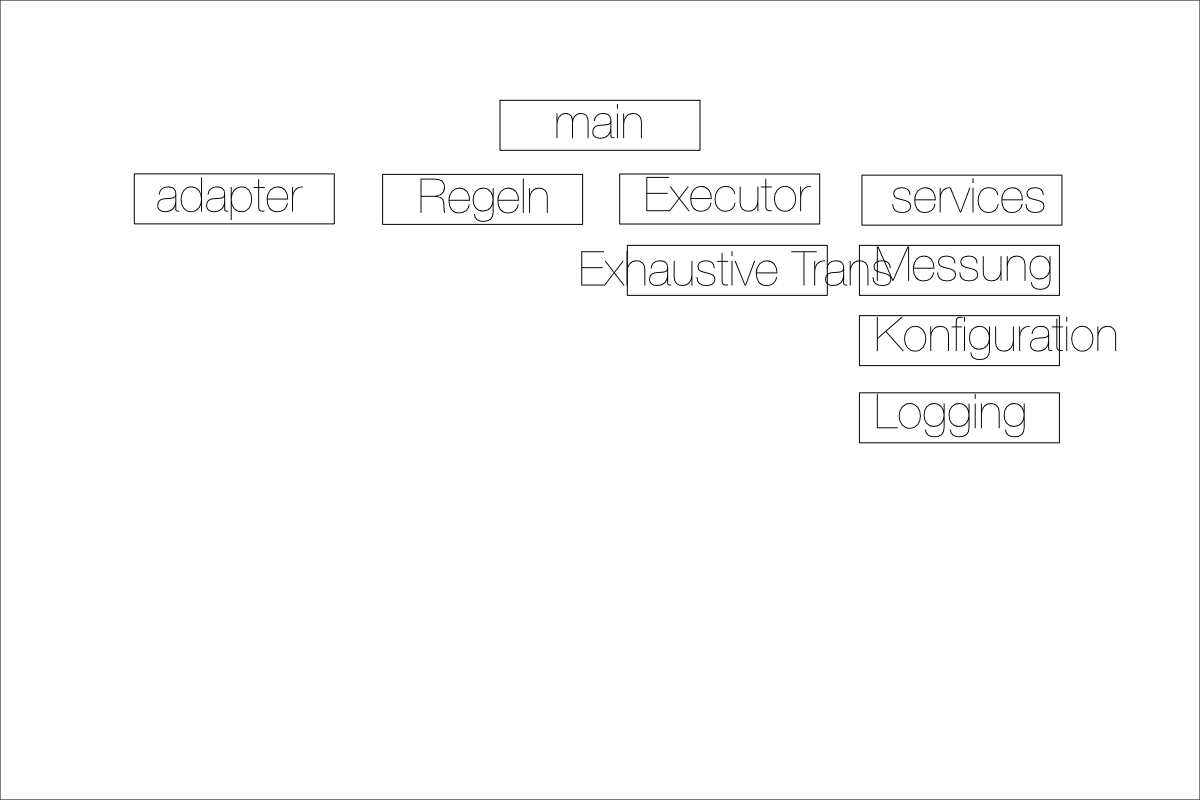
\includegraphics[width=\textwidth]{04_Implementierung/Matrix.png}
  \caption{Projektorganisation}
  \label{ProjectOrga}
\end{figure}

Bei der Ausführung eines Tests  müssen alle Bereiche zusammenarbeiten. Der Service-Bereich und insbesondere das Konfigurationsmodul sind für die konkrete Zusammenstellung der für den Test notwendigen Komponenten verantwortlich. Er entscheidet, welche Regeln zum Einsatz kommen, welcher Exector gewählt wird, welche konkreten Pläne getestet und mit Hilfe welcher Adapter die Daten ein-  bzw. ausgegeben werden. Um zu verstehen, welche Möglichkeiten das implementierte System bietet, sind die einzelnen Komponenten im Folgenden im Detail beschrieben.


\section{Services}

Da für die Ausführung des Programms unterschiedliche Dienstleistungen benötigt werden, die auch in anderen Kontexten relevant sein können, falls das Projekt diese Funktionen im Bereich Services zusammen. Teil des Bereichs ist der Konfigurator, der die Konfiguration der Tests übernimmt, die Zeitmessung und Das Logging von Informationen.

Nicht alle Komponenten wurden selbst entwickelt, beispielsweise wurde beim Logging auf die existierende Library easylogging++ gesetzt.

\subsection{Konfiguration}


\begin{figure}[ht]
  \centering
  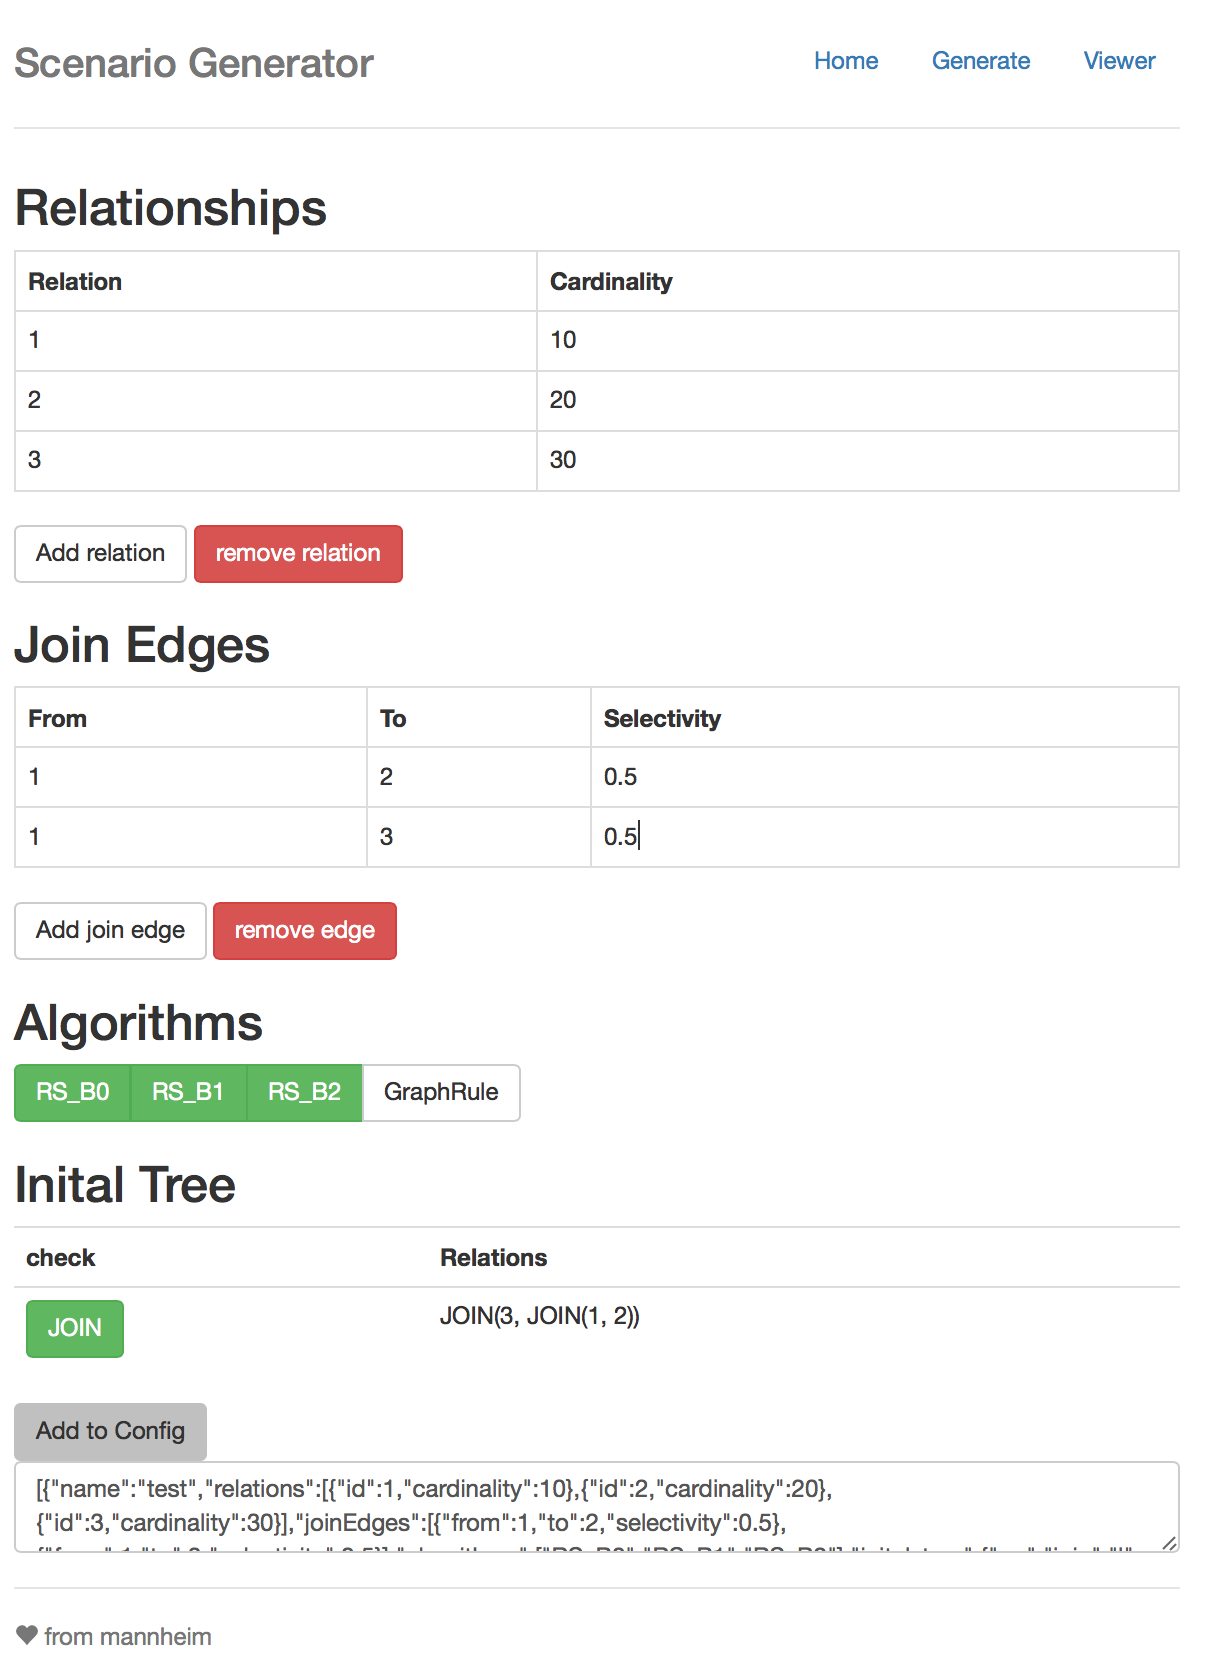
\includegraphics[width=0.5\textwidth]{04_Implementierung/ScenarioGenerator.png}
  \caption{Konfigurationstool: Scenario-Generator}
  \label{ScenarioGenerator}
\end{figure}

Das Konfigurationsmodul besteht aus zwei Komponenten. Auf der einen Seite eine Javascript-HTML Anwendung zur Generierung von Test-Szenarien (vgl. Abb. \ref{ScenarioGenerator}). Mit Hilfe dieser Anwendung können Konfigurationsfiles für den späteren Test erstellt werden. Dieses Konfigurationssystem, das in  zu sehen ist, bietet dem Nutzer die Möglichkeit Relationen mit Kardinalitäten zu erzeugen, Selektivitäten festzulegen und schlussendlich einen initalen Query Tree zu erzeugen. Ebenfalls ist es möglich die verschiedenen Regelsets, die geprüft werden sollen, festzulegen.
Das Ergebnis dieses Moduls ist eine Konfigurationsdatei im JSON Format. Das Tool unterstützt die Erzeugung mehrerer Secenarios in einem Konfigurationsfile. So können mehrere Scenarios in einem Test-Run durchgespielt werden.

Die eigentliche Konfiguration findet in C++ statt. Mit der Library json11 \cite{json11} wird das Konfigurationsfile gelesen. Für jedes Szenario und jedes Regelset wird ein initaler Baum aus Äquivalenzklassen und Planknoten mit einem JSON-Adapter gebildet. Der Exekutor wird gewählt und mit einem Regelset initialisiert. Der initiale Baum wird dem Exekutor übergeben. Nachdem die Regeln angewendet wurden, startet der Konfigurator die Kostenschätzung. Nachdem alle Szenarios abgearbeitet sind, ist das Programm beendet.

\subsection{Zeitmessung}
Wie bereits in Abb. \ref{Ablauf} dargestellt wird die Zeitmessung nach der Konfiguration gestartet. Sobald alle Pläne expandiert sind und die Kosten berechnet sind wird die Messung beendet. Um eine möglichst genaue Messung durchführen zu können, wurde die Uhr \texttt{std::chrono::steady\_clock} verwendet. Diese Uhr ist Teil von C++11. Wie in der Dokumentation \cite{cppreference_2015_clock} beschrieben handelt es sich bei der Uhr um eine monotone Uhr. Die Uhr kann nicht rückwärts laufen, solange die physische Zeit fortfährt. Die Uhr selbst mit der Wall\-Clock\-Time verbunden und ist das passende Werkzeug zur Messung von Intervallen. 

Die Dauer zwischen Start der Expansion und dem Ende der Kostenberechnung wird in Nanosekunden gemessen, um ein möglichst akkurates Ergebnis zu erhalten. Die gemessenen Ergebnisse werden sowohl als Debug-Log in der Konsole ausgegeben, aber auch in einem Log File gespeichert.



\subsection{Logging und Debugging}

Auch zum Debugging wurde eine externe Bibliothek eingesetzt: EasyLogging++ \cite{easylogging}, ein einfach zu bedienendes jedoch hochgradig konfigurierbares Logging Instrument. Gerade die Leichtgewichtigkeit - das Tool besteht nur aus einer Headerklasse -, die einfache Bedienung und Geschwindigkeit gabem den Ausschlag zur Nutzung der Library. Mit Hilfe dieser Library werden debugging Informationen geschrieben, aber auch Zeitmessungen gespeichert, pläne ausgegeben und sonstige Debugging Nachrichten ausgegeben. Insbesondere ist die Unterscheidung zwischen unterschiedlichen Debug\-Leveln wichtig. Auf mehreren Ebenen (INFO, WARNING, DEBUG, etc.) können Informationen ausgegeen werden. Je nachdem welches Level angesprochen ist, werden nur Informationen über dieses ausgegeben. 


\section{Adapter}

Die Implementierung bietet mehrere Adapter, die zur Umwandlung von externen Formaten in eine interne Repräsentationsform oder von einer internen Repräsentationsform in ein externes Format genutzt werden können. Sie bieten die Möglichkeit andere Systeme an das bestehende System anzudocken und sorgen so für den notwendigen Anschluss und die Erweiterbarkeit durch Dritte.

Insgesamt werden drei Adapter mitgeliefert. (1) JSON\-Adapter, (2) String\-Adapter, (3) DOT\-Adapter.

Der Json-Adaper erlaubt des Daten im JSON Format zu importieren und wird beim einlesen des initalen Plans genutzt. Er wandelt auf Basis des Konfigurationsfiles JSON in Planknoten und Äquivalenzklassen um, die dann weiterverarbeitet werden können. Ebenfalls ist es möglich Pläne in JSON auszugeben. Zu diesem Zweck implementiert der Parser auch eine \texttt{dump} Methode.

Neben dem JSON\-Adapter wird auch ein String Adapter verwendet. Er ist für die Ausgabe von Plänen als String verantwortlich. Im Gegensatz zu einem JSON\-Adapter ist die Eingabe von Plänen mit Hilfe dieses Moduls nicht möglich. Auch der DOT\-Adapter erlaubt nur die Ausgabe von Plänen im DOT\-Format. Das zur Generierung von graphischen Ausgaben verwendet werden kann.

Eine weitere Aufgabe eines solchen Adapters kann auch die Übersetzungen von Relationsnamen in Bitvektoren sein. Da das vorliegende System, wie in \ref{sec:Bitvector} beschrieben, Relationen als Bitvektoren abbildet, mag es nützlich sein, Relationsnamen in Bitvektoren zu übersetzen. Für diese Übersetzung sind auch Adapter vorgesehen, die zusätzlich implementiert werden können.




\section{Regeln und Regelsets}

\subsection{Regeln}

\subsection{Regelsets}


\section{Relationen, Planknoten und Äquivalenzklassen}

\subsection{Verwaltung von Relationen}
\label{sec:Bitvector}


\begin{figure}[ht]
  \centering
  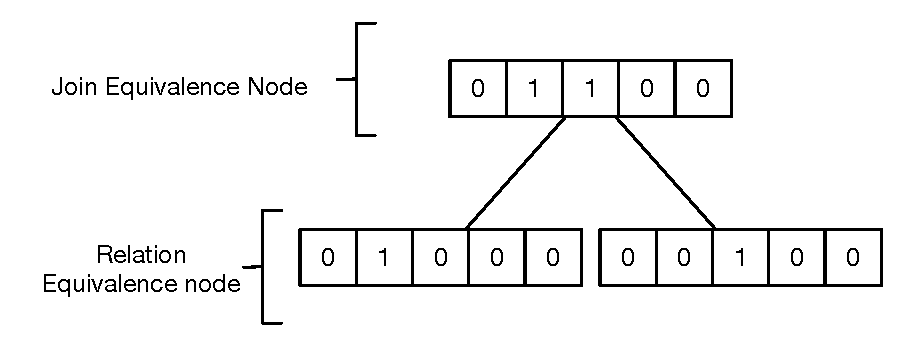
\includegraphics{04_Implementierung/Bitvector.pdf}
  \caption{Bitvekotren als Repräsentation von Relationen oder Joins}
  \label{Bitvektor}
\end{figure}

Die einzelnen Relationen werden mit Hilfe von Bitvektoren repräsentiert. Ein Bitvektor sind mehrere Bits, die entweder $TRUE$ also $1$ oder $FALSE$ also $0$ sein können. Ist das n-te Bit eines Bitvektors gesetzt, so repräsentiert dieses Bit die n-te Relation. Beispielsweise bezeichnet der Bitvektor $010000000$ die Relation mit dem Namen $1$. Mit Hilfe des Bitvektors können auch mehrere Relationen gespeichert werden $01010000000$ bezeichnet folglich die Relation mit dem Name $1$ und die Relation mit dem Namen $3$. Für die durchgeführten Berechnungen ist es nicht notwendig, dass eine Relation mit ihrem tatsächlichen Namen bekannt ist. Es reicht eine Bezeichnung mit Hilfe von Nummern aus.

Vorteil für die Verwendung von Bitvektoren ist, dass einfach Mengenoperationen durchgeführt werden können. So kann einfach geprüft werden, ob Äquivalenzklassen gemeinsame JOIN Kanten besitzen oder neue Relationen einer Äquivalenzklasse hinzugefügt werden. (vgl. Abb. \ref{Bitvector}) Dies ist besonders effizient, da nur Bits und keine komplexen Objekte wie Strings verarbeitet werden müssen.


Für externe Systeme kann es daher notwendig sein, dass Relationsnamen mit Hilfe eines Adapters übersetzt werden. Die genau Funktionsweise eines solchen Adapters wird in diesem Kapitel genauer beschrieben.




\subsection{Planknoten und Äquivalenzklassen}





\begin{figure}[h]
  \centering
  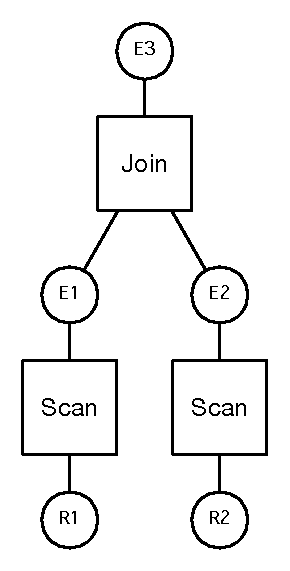
\includegraphics{04_Implementierung/JoinScan.pdf}
  \caption{Planknoten und Äquivalenzklassen}
  \label{PlanAequi}
\end{figure}

Zu  Beginn steht die Struktur in der Pläne gespeichert werden. Diese Struktur wird durch andere Komponenten bearbeitet und ausgewertet und stellt somit das Werkstück bei der Verarbeitung dar.

Ähnlich wie in anderen System kommen in der aktuellen Implementierung Äquivalenzklassen und Planknoten zum Einsatz. Äquivalenzklassen repräsentieren ein Set von unterschiedlichen, jedoch äquivalenten Planknoten. Mit Hilfe von Äquivalenzklassen und Planknoten kann die Information über alle möglichen Äquivalenten Pläne gespeichert werden. Sie können also den gesamten Search Space abbilden.
 Aufgabe eines Planknotens ist es einen Operator zu repräsentieren. Jeder Operator kann mehrere Parameter besitzen. Im konkreten Fall sind zwei Operatoren implementiert: JOINs und SCANs. Scans zeichnen sich dadurch aus, dass sie immer genau eine Relation lesen. Folglich haben Sie nur einen Parameter, um die Relation zu übergeben. Bei Joins gibt es immer genau zwei Parameter. Beide Parameter repräsentieren Datenströme, die mit Hilfe des Joins in einen gemeinsamen Datenstrom kombiniert werden.

Die kleinste im System mögliche Datenstruktur ist ein Scan. Er besteht aus einer Äquivalenzklasse, die die Relation repräsentiert. Auf sie wird ein Planknoten angewendet mit dem Operator SCAN. Dieser Planknoten ist selbst wieder Teil einer Äuqivalenzklasse. Eine solche Datenstruktur ist im linken Teil der Abbildung \ref{PlanAequi} zu finden.

Kombiniert man zwei dieser SCANs mit einem JOIN so erhält man die kleinste mögliche Struktur, die einen JOIN beinhaltet. Dies ist in Abb. \ref{PlanAequi} zu sehen. In diesem konkreten Fall ist noch keine Transformation auf den bestehenden Graphen angewendet worden. Es existieren also noch keine alternativen Planknoten. Eine solche Transformation könnte beispielsweise zur Folge habe, dass neben dem bisher bestehenden JOIN Knoten ein neuer JOIN Knoten erzeugt wird, der die beiden untergeordneten Relationen in umgekehrter Reihenfolge joint.


\subsection{Konkrete Implementierung}

Die konkrete Implementierung der Äquivalenzklasse sieht vor, wie in Abb. \ref{EquivalenceClassDiagram} zu erkennen, dass für jede Äquivalenzklasse die darin aggregierten Relationen sowie deren Nachbarn gespeichert werden. Ebenfalls wird der erste, letzte und kosteneffektivste Planknoten gespeichert. Außerdem kann festgehalten werden, ob eine Äquivalenzklasse bereits $explored$, also erforscht, ist. 






\subsection{Exektuoren}










\section{Regeln und Regelsets}


Eine entscheidende Komponente sind Regeln und Regelsets. Mehrere Regeln werden in einem Regelset zusammengefasst. Ein Regelset ist eine Instanz der abstrakten Klasse $RuleSet$, die die Methode $getRules()$ vorgibt, mit deren Hilfe ein Vektor von Regeln ausgegeben wird. Je nach Regelset können andere Regeln vorhanden sein.







\subsubsection{Organisation von Regeln}


\begin{figure}[h]
  \centering
  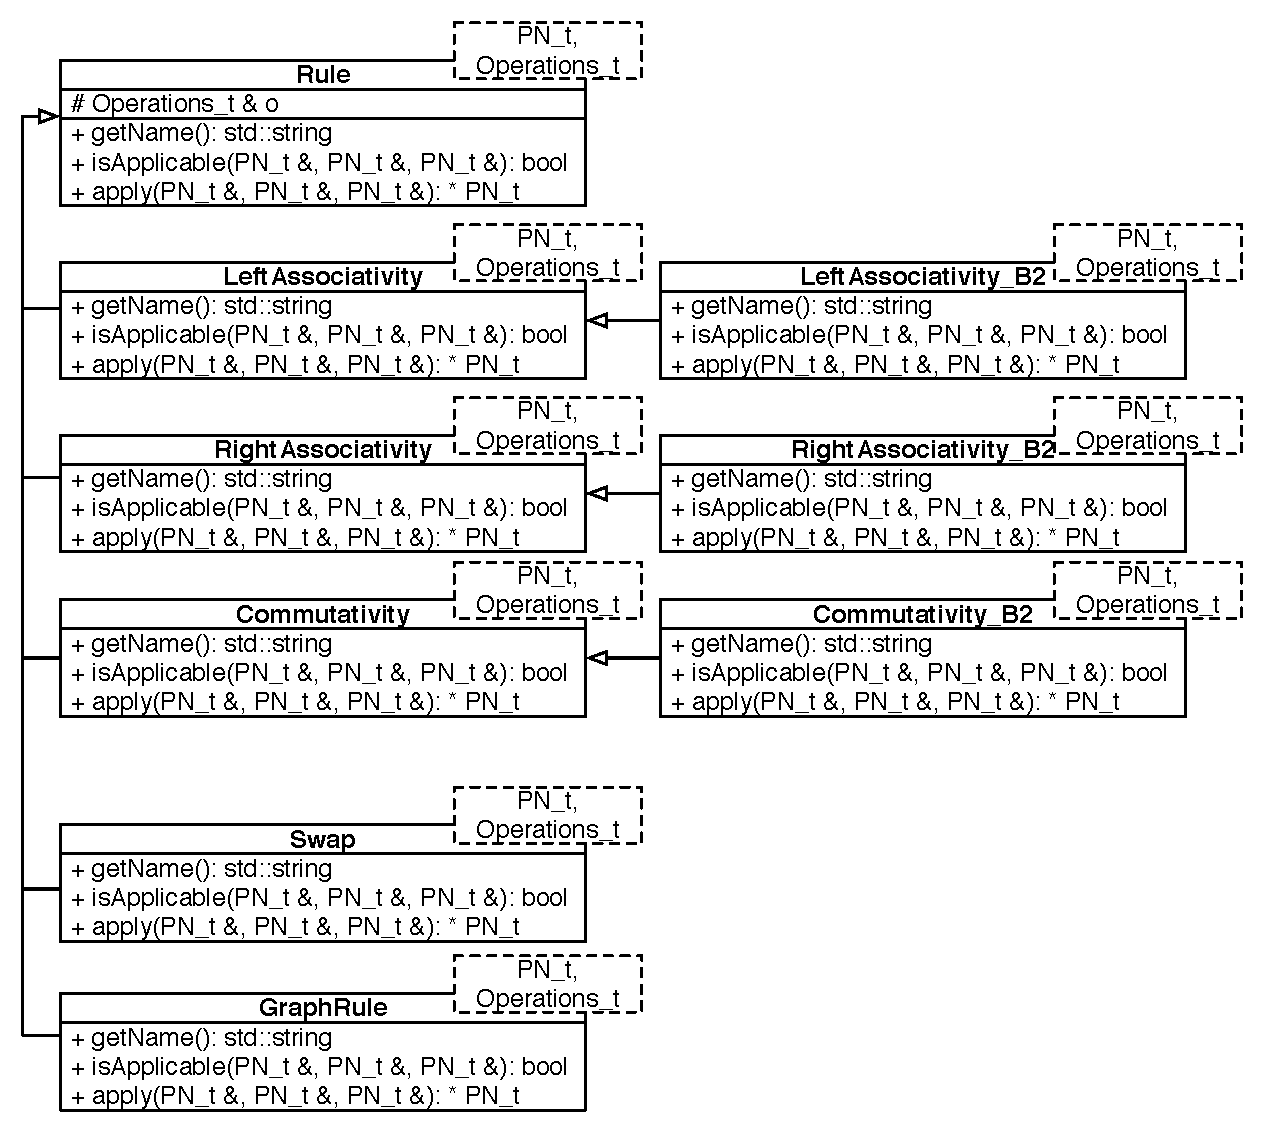
\includegraphics[width=\textwidth]{04_Implementierung/Rules.pdf}
  \caption{Regeln und Regelsets Klassendiagramm}
  \label{RuleClassDiagram}
\end{figure}


Auch bei den Regeln erben alle Regeln direkt oder - und das ist neu - indirekt von der Klasse $Rule$. Die Organisation der Klassen ist in Abb. \ref{RuleClassDiagram} dargestellt. Insgesamt wird zwischen den Regeln auf drei Ebenen unterschieden: 

$Commutativity$, $LeftAssociativity$ und $RighAssociativity$ bilden die erste Ebene der Regeln. Sie kommen in Verbindung mit den RuleSets $RS_0$ und $RS_1$ zum Einsatz.

Auf dem zweiten Level, diese Klassen sind mit dem Zusatz $B2$ gekennzeichnet, finden sich $Commutativity_B2$, $LeftAssociativity_B2$, $RighAssociativity_B2$ und $Exchange_B2$. Diese Regeln sind für das Regelset $RS_2$ notwendig und erlauben es andere Regeln zu deaktivieren. Da die Deaktivierung von Regeln eine Erweiterung darstellt, erben Kommutativität und Assoziativität von ihren Verwandten aus $RS_0$ bzw. $RS_1$. Da die Exchange Regel neu hinzukommt, erbt diese direkt von Rule.

Auf dem dritten Level findet sich die $GraphRule$. Sie ersetzt andere Regeln und ist im RuleSet $GraphRuleSet$ abgebildet.


Ähnlich wie bei Starburst bestehen Regel aus zwei Teilen. Auf der einen Seite wird geprüft, ob eine Regel zur Anwendung kommen kann. Dies geschieht mit der Methode $isApplicable$ auf der anderen Seite gibt es die Methode $apply$, die immer einen äquivalenten Planknoten zurückliefert. Mit Hilfe dieses Prinzips wurden alle Regeln implementiert. Das einheitliche Interface erlaubt es, dass Regeln in Regelsets gebündelt werden können.


\subsubsection{Erweiterbarkeit von Regeln}

Die Erweiterbarkeit ist auf mehreren Ebenen sichergestellt. Auf der einen Seite können neue Regeln erzeugt werden. Sobald diese die Form der abstrakten Klasse $Rule$ übernehmen, können sie in Regelsets zum Einsatz kommen. Ein Beispiel für eine solche Erweiterung ist die Regel $GraphRule$. Sie wurde später der entwickelten Lösung hinzugefügt. Das neue RuleSet $GraphRuleSet$ beinhaltet in diesem speziellen Fall nur eine Regel.

Eine weitere Möglichkeit zur Erweiterung wurde ebenfalls von $GraphRule$ genutzt. GraphRule gibt nicht nur einen einzelnen neuen Planknoten zurück, sondern übergibt gleich einen vollständig expandierten Baum. Auch diese Anforderung konnte ohne Veränderung des Interfaces umgesetzt werden. Da der Planknoten ein $next$ Attribut besitzt, das den vorhergehenden mit dem nächsten Knoten verbindet, können Ketten von neuen Knoten gebildet werden. Diese Ketten werden im Falle der $GraphRule$ zurückgegeben ohne dabei das Interface zu brechen.

Neben den vorgegebenen  Methoden können auch weitere Methoden für eine Regel implementiert werden. Dies ist beispielsweise bei $GraphRule$ notwendig gewesen. Hier ist es erforderlich, dass der Graph zuerst partitioniert wird, dann ConnectedComponents gefunden und schlussendlich ein Baum zurückgegeben wird. Auch dies ist innerhalb der Rules möglich.

Eine weitere Möglichkeit zur Erweiterung ist durch Templates gegeben. Template ist eine Funktion von C++ mit deren Hilfe Funktionen und Klassen mit generischen Typen arbeiten können. Dadurch ist es einer Funktion der einen Klasse möglich viele unterschiedliche Typen zu unterstützen ohne die Funktion oder die Klasse bearbeiten zu müssen. Im konkreten Fall der Regeln werden zwei dieser generischen Typen verwendet: $PlanNode$ und $Operations$. Es wird somit möglich die Klassen des Planknotens und die möglichen Operationen, die für diese Planknoten möglich sind zu ersetzen, ohne Funktionen und Klassen verändern zu können.

\subsubsection{Erweiterbarkeit von Regelsets}

Auch die Erweiterung von Regelsets ist möglich. Mit Hilfe neuer Regelsets, kann eine neue Reihenfolge bei der Ausführung definiert werden. Eine weitere Priorisierung von Regeln ist bisher nicht vorgesehen. Es ist jedoch möglich mit Hilfe der Methode $getRules()$, die für jedes Regelset implementiert ist, eine spezielle Priorisierung zu implementieren. 

Neben der Priorisierung sind auch neue Zusammenstellungen möglich. Beispielsweise ist der Unterschied zwischen $RS_0$ und $RS_1$ nur, dass eine Assoziativ-Regel weggelassen wurde. Ein Mix von alten und neuen Regeln ist möglich.

Wird ein neues Regelset erstellt, ist es nicht nur notwendig eine neue Regelset Klasse zu erstellen, sondern auch diese für das Ausführen im Executor anzumelden. Der Executor muss also ebenfalls angepasst werden.



\subsection{Ausführung von Regeln}

Das eigentliche Ausführen der Regeln wird durch einen XY durchgeführt. Im konkreten Fall kommt hier der Algorithmus ExhaustiveTransformation zum Einsatz. Der Algorithmus startet mit einer Äquivalenzklasse. Innerhalb dieser Äquivalenzklasse werden die Regeln, die durch ein Regelset vorgegeben sind auf einem PlanKnoten ausgeführt. Die Ausführung geschieht hierbei zuerst auf den Oberen Ebenen und setzt sich dann auf den Kindern eines Knoten fort. Somit können bei der Transformation eines gegebenen Baums alle Regeln auf andere Bäume angewendet werden.

Wichtig ist hierbei zu bemerken, dass dieser Algorithmus immer zuerst prüft, ob eine Regel auch tatsächlich für die Anwendung geeignet ist und dann erst der Algorithmus ausgeführt wird. Neben der eigentlichen Eignung wird auch geprüft, ob eine Äquivalenzklasse bereits vollständig expandiert wurde. Falls dies der Fall ist, wird von einer weiteren Anwendung von Regeln abgesehen. Diese Funktion kann insbesondere Vorteile bei der Implementierung von neuen Regelsets bieten. Nutzt ein gegebenes Regelset die Möglichkeit nicht nur einen neuen Planknoten zu generieren, sondern gleich mehrere Planknoten zu erstellen und auch in diesem Zusammenhang bereits mehrere Kinder-Knoten zu erstellen, kann die Reihenfolge der Expansion von Äuqivalenzklassen geändert werden. Die einzelnen Äquivalenzklassen, die bereits durch eine Regel expandiert wurden, werden als solche markiert und die bisher vorhandenen Regeln werden nicht mehr ausgeführt.


\section{Kostenschätzung und statistische Informationen}



Die Kostenschätzung zur Suche des optimalen Plans geschieht bei der vorliegenden Implementierung in einem eigenen Kostenschätzungsmodul.Teil des Kostenmoduls ist ein Katalog innerhalb dessen Informationen über Selektivität von JOINs und Kardinalitäten von Relationen gespeichert sind. Diese Informationen werden aus dem Katalog mit Hilfe des Kostenschätzers ausgelesen und die Kosten für einen Planknoten berechnet.

Die Berechnung der Kardinalität findet bottom up statt. Für jede Äquivalenzklasse wird die optimale Kardinalität berechnet und gespeichert. Der Planknoten mit dessen Hilfe diese optimale Kardinalität erreicht wird, wird als bester Planknoten markiert. Folgt man dem Pfad der besten Planknoten ergibt sich der kostenoptimale Baum an Planknoten. Die Berechnung sieht vor, dass immer die Selektivität eines Operators mit dem Produkt der Kardinalität der Eingabeparameter multipliziert wird. Beispielsweise wird auf der untersten Ebene - der Ebene der Scans - für eine gegebene Relation die Kardinalität mit der Selektivität von 1 multipliziert, da die gesamte Relation verarbeitet werden muss. Bei einem Join können komplexere Situationen auftreten. Zuerst wird das Produkt der Kardinalität der Eingabe Parameter berechnet. Diese kann dann mit der 
Selektivität multipliziert werden. Das Produkt der Kardinalitäten repräsentiert in diesem Falle die Kardinalität des möglichen Kreuzproduktes, das mit Hilfe von Selektoren eingeschränkt wird.



\subsection{Zusammenfassung}

Gerade im Bereich der Regeln ist klar zu erkennen, dass die SOLID Prinzipien eingehalten wurden. Hier ist jede Klasse nur für genau eine Aufgabe zuständig. Ein hohes Maß an Kohäsion konnte erreicht werden. Die Regelklassen  sind offen für Erweiterungen, jedoch geschlossen für Modifikationen. Dies wird insbesondere bei der Erweiterung mit Hilfe des Regelsets $GraphRuleSet$ deutlich. Auch das Liskov Substitutionsprinzip wurde eingehalten. Alle Klassen verhalten sich nach außen gleich und liefern dasselbe Ergebnis, einen Planknoten, zurück. 
\subsection{Search Space}

Der Suchraum (Search Space) bildet die Grundlage für die Suche nach einem optimalen Plan. Innerhalb des Suchraums findet die Auswahl des optimalen Plans statt. 
Zuerst wird der Search Space erforscht. In einem zweiten Schritt werden die alternativen Pläne bewertet. Am Ende wird der optimale Plan ausgeführt.



Als Search Space wird die Menge der logisch äquivalenten Pläne, die auf Grund einer Anfrage gebildet werden können, bezeichnet. Die Menge der äquivalenten Pläne kann so mächtig und so groß sein, dass nicht alle äquivalenten Pläne mit Hilfe von bekannten Techniken gefunden werden können. Der Search Space, der mit Hilfe dieser bekannten Mittel gefunden werden kann, wird als potenzieller Suchraum (Potential Search Space) bezeichnet. Die Pläne, die innerhalb dieses Search Spaces liegen, werden auf Grund ihrer Erreichbarkeit auch als accessable bezeichnet. Die Menge der Pläne, die nicht gefunden werden können, heißen folglich non-accessable. Da selbst die Menge der Pläne des Potential Search Spaces sehr groß sein kann, berechnen Anfragenoptimierer i.d.R. ihre Suche nach Planalternativen ab. Die Menge der tatsächlich gefundenen Alternativen wird als tatsächlicher Suchraum (Actual Search Space) bezeichnet.


\begin{figure}[h]
  \centering
  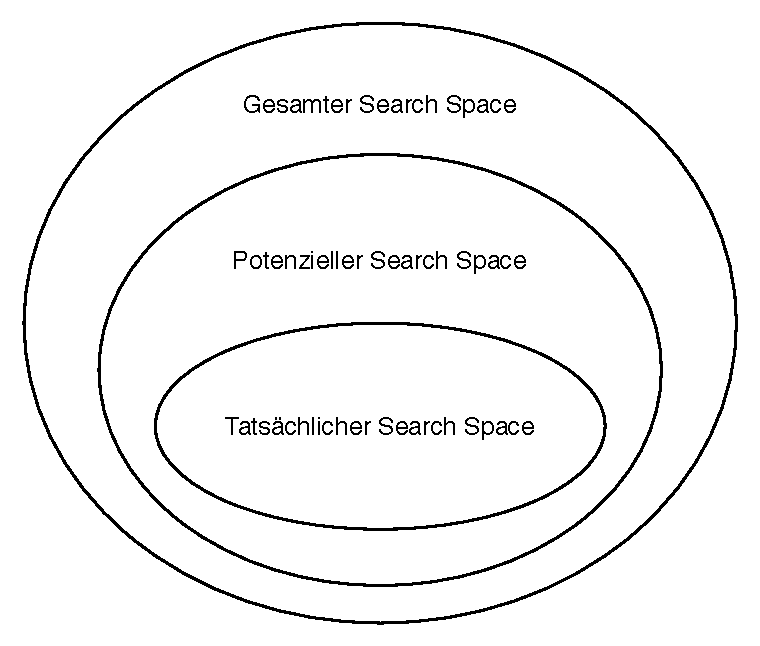
\includegraphics{02_Grundlagen/SearchSpace.pdf}
  \caption{Search Space}
  \label{SearchSpace}
\end{figure}

In Abbildung \ref{SearchSpace} ist der optimale Fall eines Search Spaces zu sehen. Der Actual Search Space ist ein Subset des Potential Search Spaces und dieser wiederum ein Subset des gesamten Search Spaces. In der Realität sind auch andere Formen möglich. Der Search Space kann beispielsweise durch eine fehlerhafte Implementierung Pläne dem Actual Search Space zuordnen, die selbst nicht Teil des gesamten Search Spaces sind.

Um einen Search Space zu erforschen,  kommen Enumeratoren zum Einsatz. Diese werden im nächsten Abschnitt genauer behandelt.
\subsection{Enumeratoren}



Enumeratoren sind für die Erforschung eines Surchraums verantwortlich. Sie generieren basierend auf einer Anfrage unterschiedliche alternative Pläne. Es lässt sich im Allgemeinen zwischen zwei Klassen an Enumeratoren unterscheiden: dynamisch programmierte und regelbasierte Enumeratoren.  \todo{Quelle}

Das Konzept der dynamischen Programmierung wurde zuerst durch IBM's System R umgesetzt \cite{selinger1979access}. In diesem System wird die Reihenfolge der JOINs, die für eine Anfrage notwendig sind verändert, um die Anfrage zu optimieren. Der Search Space, der durch den Enumerator erforscht wird, besteht aus Join Trees. Je nach Enumerator werden nur bestimmte Join Trees behandelt, die im Weiteren kurz erklärt werden.

Je nach \ac{DBMS} kann sich ein Enumerator nur auf einen Teil des gesamten Search Spaces beschränken. So ist es möglich, dass eine Beschränkung auf Grund der Form eines Baumes gebildet wird. Grob lässt sich wie in Abb. \ref{TreeTypes} zu sehen ist, zwischen drei Arten an Bäumen unterscheiden, Left-Deep, Busy und Right-Deep Trees. Je nach behandelter Join Art werden mehr oder weniger potenzielle Bäume aus dem Suchraum ausgeschlossen. Je nach Größe des potentiellen Suchraums kann sich die Suche effizienter oder weniger effizient gestalten. Einige \ac{DBMS}e argumentieren, dass die Beschränkung auf beispielsweise left-deep trees vorteilhaft wäre, da Aufwand für die Suche nach den Plänen gespart werden kann und trotzdem eine große Menge an alternativen Plänen erzeugt wird, die für sich genommen auch einen Plan nahe dem optimalen Plan bilden. 
\subsection{Kostenschätzung}

Um den optimalen Plan zu finden, müssen die Kosten für einen Plan bewertet werden. Diese Kostenabschätzung geschieht in einer Cost-Estimation \cite{bruno2011automated}. 

Die Kosten einer Datenbankabfrage sind von mehreren Faktoren abhängig. Um eine Grundlage für den Vergleich von verschiedenen Plänen zu haben, müssen die Kosten für jeden einzelnen Plan abgeschätzt werden. Die Kosten für die gesamte Abfrage setzten sich dabei aus den Kosten für die Enumeration der Anfrage, der Berechnung der Kosten und der Ausführung der eigentlichen Anfrage zusammen. Da die Kosten für Enumeration und Cost-Estimation für jeden Plan gleich sind und die Kosten für die Berechnung verglichen zu den Kosten des Auslesens der Daten wenig signifikant sind \cite{selinger1979access}, kann das Augenmerk auf die Abschätzung der Kosten der Ausführung gelegt werden.

Bei der Ausführung einer Anfrage sind vor allem die CPU, die Eingabe / Ausgabe und Arbeitsspeicherkosten entscheidend. Die Kosten können für jede dieser Ressourcen getrennt oder gemeinsam betrachtet werden. Die Kostenabschätzung muss insgesamt jedoch akkurat sein, da der Anfrageoptimierer nur so gut sein kann, wie es der Kostenschätzer erlaubt. Die Berechnung der Kosten geschieht i.d.R. nach folgender Maßgabe:

\begin{enumerate}
\item Statistische Informationen werden gesammelt
\item Für einen Operator im \ac{QEP} werden die Informationen aus Subbäumen berechnet und zusammengezählt
\end{enumerate}

Bei der Sammlung statistischer Informationen können neben der Kardinalität von Relationen, der Selektivität von Operatoren und andere Werte vorkommen. Falls noch keine Werte über ein bestimmtes Datum gesammelt wurde, werden i.d.R. Standardwerte angenommen. Am Ende ist der Plan optimal, der die niedrigsten Kosten aufweist. Einige Datenbanksysteme setzten bei der Berechnung der Kosten auf das Optimalitätsprinzip von Bellman \cite{Bellman:1957}, das aussagt, dass eine optimale Lösung immer aus optimalen Teillösungen besteht. Dieses Prinzip wird in diesem Kapitel im Abschnitt System R genauer besprochen und von Kapitel 5 Implementierung im Bereich der Kostenschätzung aufgegriffen.






\subsection{System R}

System R ist ein von IBM in den 1970er Jahren durchgeführtes Datenbank Research Projekt \cite{selinger1979access}, \cite{wade2012ibm}, \cite{chamberlin1981history}, \cite{astrahan1976system}, \cite{astrahan1978system}. Es gilt insbesondere auf Grund von zwei Aspekten als der Pinoneer für moderne Datenbanksysteme: Auf der einen Seite wurde in System R zum ersten Mal \ac{SQL} implementiert. Auf der anderen Seite war es das erste System, das die Leistungsfähigkeit von relationalen Datenbanksystemen unter Beweis stellte. Fundamentale Design Entscheidungen, wie dynamische Programmierungsalgorithmen für \ac{QO}, prägen die weitere Entwicklung von Datenbanksystemen. System R gilt als der Vorgänger von IBMs DB2 und als Grundlage für viele andere Datenbanksysteme.


\subsubsection{Architektur und Systemstruktur}

\begin{figure}[h]
  \centering
  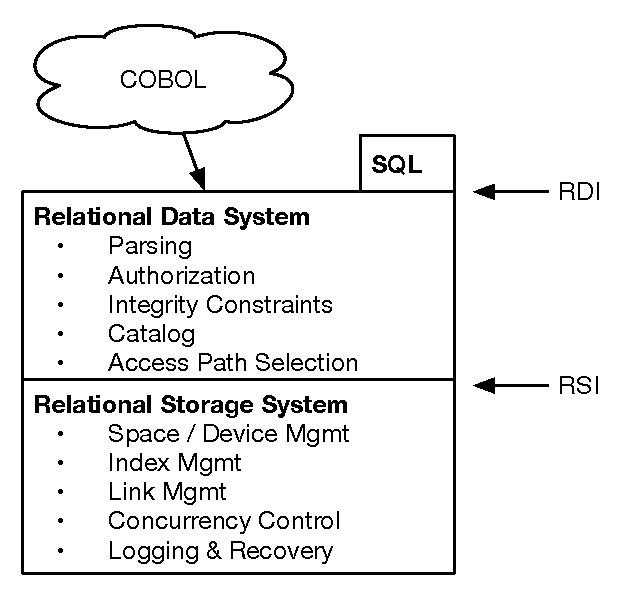
\includegraphics{03_Related_Work/SystemR.pdf}
  \caption{System R Architektur \cite{astrahan1976system} \cite{astrahan1978system}}
  \label{SystemRArchitecture}
\end{figure}


Wie in Abbildung \ref{SystemRArchitecture} zu erkennen ist,  besteht das System aus zwei Teilsystemen: \ac{RSS}, das dem RTS entspricht, und \ac{RDS}, das äquivalent zu einem CTS ist.

Das \ac{RSS} ist für die physische Verwaltung der Datenbank verantwortlich. Es kontrolliert u.a. die Speicherverwaltung, das Device-Management, die Transaktionskonsistenz und die Transations- sowie System-Wiederherstellung. Im Besonderen fällt in den Aufgabenbereich der Zugriff auf einzelne Tupel von Base Relations. Diese Funktionen werden gegenüber des \ac{RDS} mit Hilfe des \ac{RSI} bereitgestellt.

Das \ac{RDS} übernimmt via \ac{RDI} die Kommunikation nach außen und leitet Befehle über das \ac{RSI} weiter. Anfragen von außen werden mit Hilfe von \ac{SQL} an das System gestellt. Es ist auch möglich, dass externe Sprachen wie Cobol verwendet werden, die ohne Weiteres mit dem \ac{RDI} kommunizieren. In diesen Fällen muss SQL nicht verwendet werden. Das \ac{RSS} wandelt die Umfrage in eine für das \ac{RSI} verständliche Form um. Über das RSI wird die Anfrage entgegen genommen und ausgeführt.




\subsubsection{Verarbeitung von Anfragen}

Wie bei anderen relationalen Datenbanksystemen steht am Beginn eine in \ac{SQL} formulierte Anfrage. Diese Anfrage wird in vier Schritten verarbeitet: Parsen,  Optimieren, Code Generierung und Ausführen.

Im ersten Schritt, Parsen, wird wie bei späteren Systemen die Syntax geprüft und die Anfrage in eine interne Repräsentation umgewandelt. Bei System R werden hierzu Query Blöcke verwendet. Sie repräsentieren die Anfrage mit einer SELECT list, einer FROM list und einem WHERE Baum. Er beinhaltet eine Liste der Elemente, die beispielsweise zum JOIN von Tabellen und der Einschränkung von Datensätzen dienen. Es ist möglich, dass mehrere Query Blöcke für eine einzige Anfrage vorhanden sind. Dies geschieht dann, wenn eine Anfrage Inner-Queries verwendet bzw. Anfragen als Argumente für eine WHERE Bedingung zum Einsatz kommen.


Sobald die Anfrage in Query Blöcke verarbeitet wurde, kommt der \ac{QO} zum Einsatz. Der Optimierer prüft zuerst, ob die genutzten Relationen und Felder auch in der Datenbank vorhanden sind und schlägt Informationen über diese im System R Catalog nach. Teil dieser Informationen sind statistische Informationen der referenzierten Relationen. Diese werden später für die Auswahl der richtigen Access Plans verwendet.

Im nächsten Schritt, optimieren, bestimmt der Optimizer für jeden Query Block den optimalen Access-Pfad. Zuerst wird die Evaluationsreihenfolge der Query Blocks im Statement festgelegt. Dann wird für jeden Query Block die FROM Relationen betrachtet. Sind mehr als eine Relation vorhanden, werden Permutationen der JOIN-Order gebildet. Es wird der Pfad mit den günstigsten Kosten gewählt und die notwendigen Modifikationen werden an der Anfrage vorgenommen. Das Resultat des Prozesses ist ein Plan in der \ac{ASL}.

Nachdem der Plan gefunden und als \ac{ASL}-Tree vorhanden ist, kommt der Code Generator zum Einsatz. Er übersetzt den \ac{ASL}-Plan in einen  Maschinencode. Dieser Code führt die Anfrage des Nutzers auf der Datenbank aus. 

Der Maschinencode wird dann auf dem \ac{RSS} über das \ac{RSI} ausgeführt und das Ergebnis zurückgegeben.

\subsubsection{Kostenberechnung}
Bei der Auswahl des optimalen Plans beginnt System R mit der Reihenfolge der Query Blocks. Zuerst wird für jeden Query Block geprüft, ob mehrere Tabellen in den FROM Listen vorhanden sind. Falls das der Fall ist, wird die Optimale Join-Order und die Methode des Joins bestimmt. Der Plan mit den geringsten Gesamtkosten für einen Block wird ausgewählt.

Zur Bestimmung der Kosten werden statistische Informationen aus dem System R Catalog herangezogen. Die Berechnung der Kosten für einen Access Plan, werden mit Hilfe der folgenden Funktion abgeschätzt:

$$Cost = Page Fetches + W * (RSI calls)$$


$Page Fetches$ repräsentieren die I/O Operationen, die beispielsweise durch den Abruf der Index Pages und der eigentlichen Pages entsteht. $RSI calls$ ist die Anzahl der erwarteten Datensätze, die durch das \ac{RSS} zurückgegeben werden. Sie dient als Abschätzung wie hoch der CPU Aufwand für die Rückgabe der Werte ist. Mit Hilfe des Parameters $W$ wird eingestellt in welchem Verhältnis I/O zu CPU Kosten stehen.


%\sout{Bei der Auswahl eines Plans unterscheidet das System zwischen einer \"interessanten\" Reihenfolge, also sortierten Ergebnissen, und einer ungeordneten Reihenfolge. Als interessante Reihenfolge, werden Reihenfolgen betrachtet, die gesamter Reihenfolge notwendig sind und die Kosten, die für das lesen in ungeordneter Reihenfolge notwendig sind und addiert auf diese Kosten, die Kosten für das Ordnen der Ergebnisse falls eine ungeordnete Reihenfolge + das Ordnen der Ergebnisse gemeinsam kürzer dauert als das direkte Ausgeben einer interessanten Reihenfolge wird sich für die günstigere Variante entschieden.}


Die Berechnung findet auf Basis der Daten statt, die von System Rs Catalog bereitgestellt werden. Die Daten umfassen folgende Kennzahlen:

\begin{itemize}
\item $R$: Kardinalität der Relation (Anzahl Tupel)
\item $D$: Anzahl der Daten-Pages, die von der Relation belegt werden
\item $T$: Durchschnittliche Anzahl der Tupel pro Daten Page (gleich $G/D$).
\item $H$: Koeffizient der CPU-Kosten ($1/H$ ist die Anzahl der Tupelvergleiche, die  als gleich den Kosten für einen Page Access sind.)
\end{itemize}

Auf Basis dieser Kennzahlen werden die Kosten je nach Operator festgestellt. 

%\sout{Die Berechnung geschieht auf Daten, die durch den Catalog bereitgestellt werden, Sie enthalten Informationen über die Kardinalität und die Anzahl der Segmente, die für das auslesen einer Relation notwendig sind, ebenfalls wird ein Selektivitätsfaktor genutzt, der das Verhältnis der Gesamtheit zur eingeschlossenen Menge der Anfrage angibt. Sprich die Menge der ausgeschlossenen Tupel.}



\subsubsection{Plan Enumerator}
Die Enumeration des System R Optimizers zeigt zwei wichtige Aspekte eines Enumerators: Auf der einen Seite die    interesting order  auf der anderen Seite  die \"dynamic Programming\". 

Dynamische Programmierung geht davon aus, dass das Kostenmodell dem Optimalitätsprinzip von Bellman \cite{Bellman:1957} gehorcht. Das Prinzip sagt aus, dass sich eine Optimallösung aus optimalen Teillösungen zusammensetzt. In unserem konkreten Fall sagt das Prinzip, dass der optimale Plan nur aus optimalen Teilbäumen bestehen kann. Somit müssen nur optimale Subplans zur Erzeugung des optimalen Plans verwendet werden i.a.w. sucht man mit Hilfe eine bottom-up Enumeration Algorithmus nach dem optimalen Plan. So müssen nur Subpläne in Betracht für eine optimale Gesamtlösung gezogen werden, die für sich optimal sind. 

Ein weiterer wichtiger Aspekt von System R ist die Verwendung von Interesting Orders. Als Interesting Orders werden Reihenfolgen, die innerhalb eines Joins entstehen bezeichnet, die zwar höhere direkte Kosten verursachen, jedoch zu niedrigeren Gesamtkosten beitragen können. So ist es möglich, dass die Kosten durch einen Nested-Loop Join zwar höher sind als durch einen Merge-Join, allerdings die Gesamtkostenbilanz durch den teureren Nested-Loop Join positiv beeinflusst wird. Gerade beim Einsatz von Prunning Algorithmen ist es möglich, dass so ein global suboptimaler Plan gewählt wird. System R identifiziert diese geordneten Resultate, die für die zukünftige Ausführung von Vorteil sein können. Außerdem werden Pläne in System R nur dann verglichen, wenn sie die selbe Reihenfolge und den selben Ausdruck besitzen. 
\section{Das Starburst Project}

Das Starburst Projekt \cite{lohman1988Starbust}, \cite{haas1989extensible}, vorangetrieben und entwickelt von IBM,  startet unter der Prämisse, dass bestehende DBMSe nicht in der Lage sind die wachsenden Anforderungen von verschiedenen, neuartigen Applikationen vollumfänglich zu entsprechen. Zur Erfüllung der individuellen Ansprüche wurde das Starburst Projekt begonnen. Sein Ziel ist es dem \ac{DBI} die Möglichkeit zu geben eine die relationale Datenbank zu erweitern und so die Bedürfnisse von spezifischen Anwendungen zu erfüllen. Beispielsweise ist es möglich neue Zugriffs- und Speichermethoden zu implementieren oder neue Join Methoden zu erstellen. Um diese Features zu ermöglichen stellt Starburst eine Anfragesprache, einen regelbasierten Optimierer, Query Rewriter und ein Ausführungssystem basierend auf relationaler Algebra zur Verfügung. Dieses Kapitel befasst sich zuerst mit der Aufteilung zwischen Ausführung und Anfrage, wie sie bereits zu Beginn dieses Kapitels besprochen wurde. Es folgt ein Überblick über die eingesetzte Regelmaschine und eine Erläuterung des Starbust Query Optimizers.

\subsection{Ausführung einer Anfrage}

Bei der Ausführung einer Anfrage mit Hilfe von Starburst wird grob zwischen zwei Phasen unterschieden: Übersetzungs- (Compile-) und Ausführungszeit (Run-Time). Während der Compile-Time wird aus der Anfrage ein Plan generiert, der zur Run-Time durch das Execution System ausgeführt wird. Der Query Optimizer findet seine Anwendung zur Compile-Time; die Query Execution Engine kommt zur Run-Time zum Einsatz.

\begin{figure}[h]
  \centering
  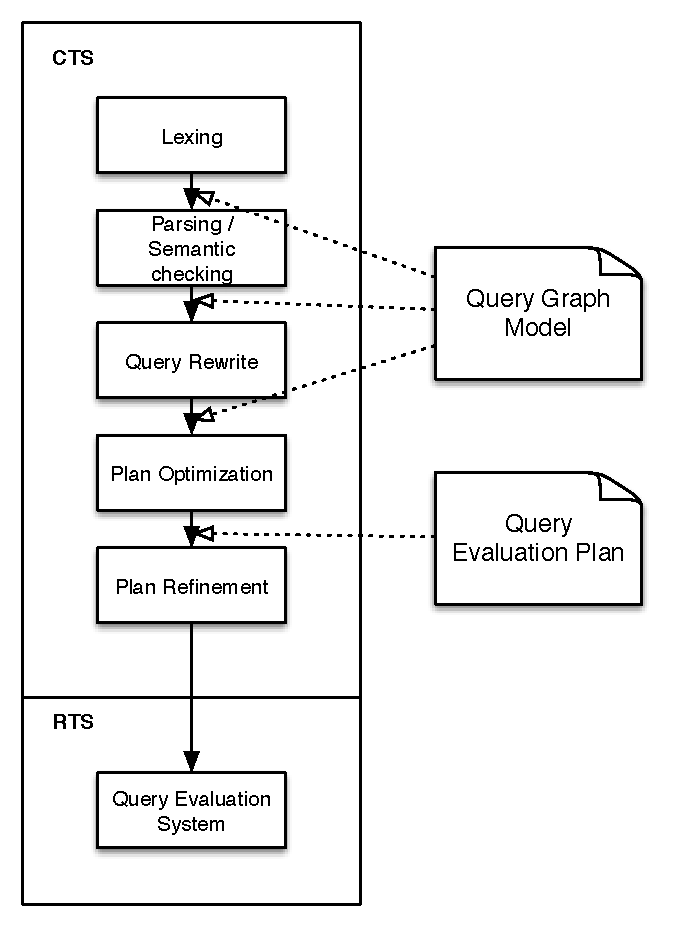
\includegraphics{03_Related_Work/StarburstFlow.pdf}
  \caption{Starburst}
\end{figure}

Zur Comile-Time wird eine gegebene Anfrage auf semantische Korrektheit geprüft und in ein \ac{GQM} übersetzt. Basierend auf diesem \ac{GQM} wird die Optimierungen der Anfrage durch zuerst einen Query Rewriter, einen Plan Optimierer und einen Plan Refiner durchgeführt.

Der Query Rewriter hat zwei konkrete Aufgaben: Auf der einen Seite soll die Anfrage in eine möglichst deklarative Form umgewandelt werden, hierbei werden insbesondere Anfragen entschachtelt. Auf der anderen Seite sollen weithin in der Forschung akzeptierte Heuristiken, beispielsweise der Push-Down von Argumenten, angewandt werden.
Bei der Planoptimierung durchläuft der Plan vom \ac{GQM} hin zu einem QEM drei Stationen. Die drei wesentlichen Aspekte sind der Plan Generator, die Berechnung der Plankosten, um den optimalen Plan auszuwählen. 

\subsection{Regel-Maschine}

Zur Ausführung von Optimierungen wurde für die Starburst Datenbank eine eigene Regel-Maschine entwickelt \cite{lohman1988Starbust}. Diese Regelmaschine ist für die Anführung von Regelsets verantwortlich, die bei der Transformation der QGMs zur Anwendung kommen und durch den \ac{DBI}  erweitert werden können. Die Regelmaschine basiert auf fünf Prinzipien:

\begin{enumerate}
\item Regel der arbiträren Komplexität: Eine Regel ist bei Starburst in zwei Teile aufgeteilt: Eine Koordinierungs- und eine Ausführungsfunktion. Bei dem Aufruf einer Regel muss zuerst geprüft werden, in wie weit die Regel angewendet werden darf. Ist sie anwendbar, wird die Ausführungsfunktion exekutiert.

\item Bei der Nutzung eines GQMs kann entweder eine Tiefen- als auch eine Breitensuche zur Anwendung kommen. Diese Art der Suche ist weder an die Regel noch an das Regel-Set geknüpft, sondern mit dem QGM selbst verbunden.


\item Die Regeln werden bei Starburst in Regelsets unterteilt. Ein Regel-Set besteht aus mehreren Regeln, die entweder sequenziell, nach einer vorab vergebenen Priorität oder einem statistischen Verfahren aufgerufen werden. Jede Regel und jedes Regel-Set kann andere Regeln und Regel-Sets als Teil einer Subroutine ausführen. Neben der Funktion der Zusammenfassung der Regeln ist es Aufgabe der Regel-Sets.

\item Um die Ausführung von Transformationen zu limitieren, insbesondere bei der Ausführung des Rewriters, kann ein Budget vorgeschrieben werden. Sobald dieses Zeitbudget aufgebraucht ist, wird die Ausführung von Transformationsregeln abgebrochen. Es ist für diese Funktion unbedingt notwendig, dass Regeln immer vollständige QGMs zurückliefern, da sonst ein unvollständiger QGM als Resultat des Optimierers entstehen kann.

\item Schlussendlich ist es dem Nutzer der Datenbank möglich zu jedem beliebigen Zeitpunkt Regeln ausser Kraft zu setzen. Dies geschieht nur für den Nutzer lokal und andere Nutzer der Datenbank sind nicht betroffen. Spezielle Anwendungsfälle können so passgenau optimiert werden.
\end{enumerate}

\subsection{Plan Optimierer}

Der Plan Optimierer generiert basierend auf einem QGM mehrere alternative Query Evaluation Plans (QEPs). Für jeden dieser QEPs werden die Kosten geschätzt und der günstigste für die Weiterverarbeitung ausgewählt. Um die Erweiterbarkeit des Optimierers zu gewährleisten wurden die drei Komponenten (Plangenerierung, Kostenschätzung und Suchstrategie) von einander soweit getrennt, dass sie einzeln erweitert und verändert werden können. 

\subsection{Starburst Plan Generator}
\emph{HIER ÜBERARBEITEN}
Der Plangenerator des Starburst Projekts, der für die Generierung von Planalternativen verantwortlich ist, bedient sich eines "Build Block"-Ansatzes[Lohm88] und einem Regel-Set, das auf einer eigenen Grammatik basiert.  

Als Build Block werden low-level-Datenbankoperationen (wie Access, Join und Sort) zu high-level Operationen kombiniert. Diese können wiederverwendet werden. Dank des Konzepts der Build Blocks ist es möglich die Erstellung und Verarbeitung in zwei wesentlichen Aspekten zu vereinfachen:


\begin{enumerate}


\item Die Regeln sind leichter von einem DBI zu lesen und zu verstehen, da die Fülle an Information mit Hilfe von Build Blocks aggregiert wurde.

\item Das Ausführen von Regeln wird effizienter. Da nicht mehr ganze Graphen nach Pattern durchsucht werden müssen, sondern direkt über Build Blocks erkannt werden, erleichtert sich die Ausführung. Ebenfalls ist es dank der Nutzung von Macro-Expandern möglich, die Geschwindigkeit zu verbessern.


\end{enumerate}


$$TEXT$$
Jede Regel erlaubt es, dass aus ihr sowohl eine als auch mehrere Graphen entstehen können. In diesem Falle spricht man von Sets von Alternativen Plänen (SAP). 


\begin{itemize}
\item LOLEPOP
\item STARs
\end{itemize}

 
\subsection{Exodus, Volcano, Cascades}

In diesem Kapitel wird der Verlauf des EXODUS Projektes und seiner Nachfolger Volcano und Cascades behandelt. Zuerst wird ein allgemeiner Überblick über den Aufbau von EXODUS gegeben. Hierauf werden die Änderungen und Erweiterungen von Volcano und Cascades besprochen. Insbesondere wird in diesem Teil auf die Art und Weise der Implementierung der Query Optimizer eingegangen. 

\subsubsection{Exodus}


Bereits in den 1970er Jahren begann Graefe mit der Implementierung eines DBMS Frameworks unter dem Titel EXODUS (EXtensible Object-oriented Database System) \cite{carey1990exodus} . Das Projekt, das die Grundlage für Volcano legen sollte, hatte sich zum Ziel gesetzt einen erweiterbaren, applikationsspezifischen und hochperformanten Baukasten zusammenzustellen, mit dessen Hilfe neue Datenbanksysteme generiert werden konnten. 

Im Gegensatz zu konventionellen DBMS wie Postgres handelt es sich bei EXODUS nicht um ein funktionsfähiges und sofort einsatzfähiges DBMS, sondern um einen Baukasten, auf dessen Basis ein neues System durch einen DBI erstellt werden kann. Im Gegensatz zu anwendungsübergreifend designten DBMS wie Postgres bietet EXODUS den Vorteil, dass eine Datenbank speziell für die Bedürfnisse eines Anwendungsfalles angepasst wird. Um dennoch das Ziel der Performance nicht aus den Augen zu verlieren, werden viele Komponenten nicht immer wieder auf einer grünen Wiese entwickelt, sondern auf dem Fundament des EXODUS Baukastens aufgebaut.

\begin{figure}[h]
  \centering
  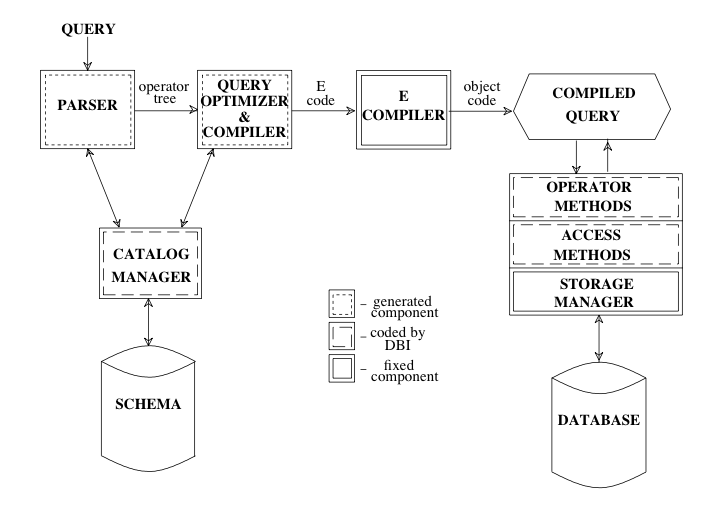
\includegraphics[width=\textwidth]{02_Grundlagen/ExodusDatabaseSystemStructure.png}
  \caption{Exodus Database System Structure}
\end{figure}

Der Baukasten von EXODUS erlaubt       besteht sowohl aus Bestandteilen, die fix vorgegeben und nicht verändert werden sollen, Bausteinen die generiert werden und Teilen, die speziell entwickelt werden müssen. Der Werkzeugkasten umfasst dabei nicht nur die Bausteine, sondern auch die Werkzeuge zur Bearbeitung und Generierung. Zu den Werkzeugen gehören ein Tool zur Erstellung eines Front-Ends für die Anfragesprache, ein Query Optimizer Generator und die Programmiersprache E (zusammen mit einem passenden Compiler). Mit Hilfe des Tools zur Erstellung eines Front-Ends für Anfragesprachen kann die Parser Komponente generiert werden. Der Query Optimizer wird als Resultat des Query Optimizer Generators erzeugt. (vgl. Fig. Exodus Database System Structure)

Neben den generierten Komponenten gibt es den E Compiler, der E Code in Objekt-Code übersetzt. Er kommt zum Einsatz, um die durch den Query Optimizer optimierte Anfrage in eine kompilierte Anfrage umzusetzen. Diese Komponente ist ähnlich wie der Storage Manager, der für die Verwaltung von Daten in der Datenbank genutzt wird unveränderlich. 

Zwischen der kompilierten Anfrage und dem Storage Manager kommen zwei Komponenten zum Einsatz, die von einem DBI geschrieben werden müssen: Die Operator Methoden und Access Methoden. Diese beiden Komponenten dienen dazu die Anfrage in Code zu übersetzen, der durch den  Storage Manager ausgeführt wird.

Bei der Implementierung eines Optimierers kommen grundsätzlich zwei mögliche Ansätze in Frage: (1) interpretierte und (2) kompilierte Programmiersprachen. Bei EXODUS wurde zuerst die Implementierung mittels sog. "AI" Sprachen versucht. In einem Prototypen wurde mit Hilfe von Prolog ein Optimierer entwickelt. Für Prolog wurde sich entschieden, da diese Sprache Pattern Matching und eine Search Engine bereitstellt. (Auch unification konnte zum Einsatz gebracht werden, um elegant Query Trees zu erstellen.) Der Hauptvorteil eines interpretierten Ansatzes war aus Sicht von EXODUS die Möglichkeit neue Regeln zur Laufzeit des Programms hinzuzufügen. Trotz dieser Vorteile wurde der Ansatz als zu langsam verworfen. Auch der Vorteil Regeln während der Laufzeit hinzuzufügen, wird in der Literatur (QUELLE) als wenig nützlich bewertet. Statt dieses Ansatzes wurde in der Folge auf die Erstellung eines Generators, der in C geschrieben wurde, gesetzt. Der Generator erstellt basierend auf Regeln einen Optimierer in C, der wiederum kompiliert werden kann. Zwar war die Entwicklung des C Generators aufwendiger als die Implementierung in Prolog, jedoch konnte auf applikationsspezifische Notwendigkeiten, wie die Implementierung von speziellen Suchverfahren, Punkt genau eingegangen werden.


Der generierte Optimierer funktioniert so, dass er den Anfragenbaum Schritt für Schritt transformiert. Die Information über bereits erstellte Baum-Alternativen wird in einer Datenstruktur namens MESH gespeichert. MESH wird außerdem genutzt um Plänge für Anfragenbäume zu speichern, die nicht beschnitten werden von der Daten Struktur. Zu jedem Zeitpunkt während der Optimiererung kann eine große Menge an weiteren möglichen Transformationen. Diese wird in der Datenstruktur \"OPEN\" gespeichert. Sie ist eine Priority Queue. OPEN ist initalisiert mit Transformationen, die auf den initialen Tree angewendet werden können. Grundsätzlich funktioniert der Algorithmus wie folgt:

\begin{lstlisting}[caption={Exekution in EXODUS}]
While (OPEN is not empty)
	SELECT a transformation from OPEN
	Apply it to the correct node(s) in MESH
	DO method selection and cost analysis for the new nodes
	Add newly enabled transformations to OPEN

\end{lstlisting}

\subsubsection{Volcano}

Volcano ist der verbesserte Nachfolger von EXODUS. Zuerst war Volcano nur ein erweiterbares, paralleles System zur Anfragenausführung. Später wurde ein neuer Anfragenoptimierer-Generator hinzugefügt. 

Der Volcano-Optimizer-Generator wurde designt und implementiert 





\subsubsection{Volcano Optimizer Generator}

Der Volcano Optimizer unterscheidet sich verglichen zu seinem Vorgänger EXODUS durch höhere Erweiterbarkeit. Er bietet Unterstützung für nicht triviale Kostenmodelle und physische Eigenschaften wie die Sortierreihenfolge von Relationen. Außerdem ist er effizienter durch die Kombination von dynamischer Programmierung, zielgerichteter Suche und “Branch-and-Bound-pruning.” Im Vergleich zu anderen regelbasierten Optimieren ist das System unabhängig von einem gegebenen Datenmodell.

\subsubsection{Volcano Optimizer Generator}

Bei der Generierung eines Plans auf Grund einer Anfrage kommt bei Volcano ein Optimierer zur Anwendung, der speziell für den Anwendungsfall generiert wurde. Der Optimierter ist das Resultat einer Model Spezifikation, die von einem Datenbank Implementierer (DBI) erstellt und durch einen Optimierer Generator in Source Code umgewandelt wird. Dieser Code wird mit Hilfe eines Compilers in das Endprodukt, den Optimierer, umgewandelt.

 \subsubsection{Design Prinzipien}

Der Optimierer folgt dabei fünf Designentscheidungen \cite{graefe1993volcano}, die die Erweiterbarkeit und eine Effiziente Suche des Optimiers erlauben.

\begin{itemize}

\item Die erste Grundlage des Volcano Optimizers ist die Anwendung von algebraischen Techniken wie algebraische Operatoren und Äquivalenzklassen. Volcano unterscheidet dabei zwischen logischer und physischer Algebra. Die Umwandlung von logischer Algebra (der Anfrage) in die physische Algebra (einem Query Evaluation Plans) geschieht bei durch die Transformation der logischen Algebra mit Hilfe von kostenbasierten Mappings von Logischen Algorithmen.


\item Das zweite Prinzip sieht vor, dass die Information über algebraische Gesetze, die zur Transformation von Algebraischen Ausdrücken genutzt werden als Regeln und Pattern modular erfasst sind. Durch dieses Prinzip sind die einzelnen Regeln klar und transparent von einander getrennt und können zu Regelsets zusammengestellt werden. Einige dieser Regelsets werden im folgenden Kapitel behandelt.


\item Das dritte Prinzip betrifft den Input des Optimierers im Gegensatz zu anderen Optimierern (namentlich Stardust) setzt der Volcano Optimizer auf algebraische Äquivalenzen als Input Parameter. Andere Systeme nutzen hier mehrere Stufen an Umwandlung, um zwischen Query und Optimizer Input zu vermitteln. 

\item Kompilierung über Interpretierung von Regeln ist das vierte Prinzip, das zur Anwendung kommt. Da es sich bei der Generierung von äquivalenten Plänen um ein CPU intensives Geschäft handelt, wurde entschieden, dass die Regeln zur Transformation der Pläne kompiliert und nicht interpretiert werden. Zwar verliert der Optimierer daduch die Möglichkeit ad hoc neue Regeln in den Optimierer aufzunehemen. Diese Möglichkeit wird jedoch in der Praxis nicht benötigt.

\item Das letzte Prinzip ist, dass der Volcano Optimierer auf dynamisches Programmieren bei der Generierung von Programmen setzt. 


\end{itemize}






\section{Oracle}
\subsection{Oracle Architektur}


\begin{figure}[h]
  \centering
  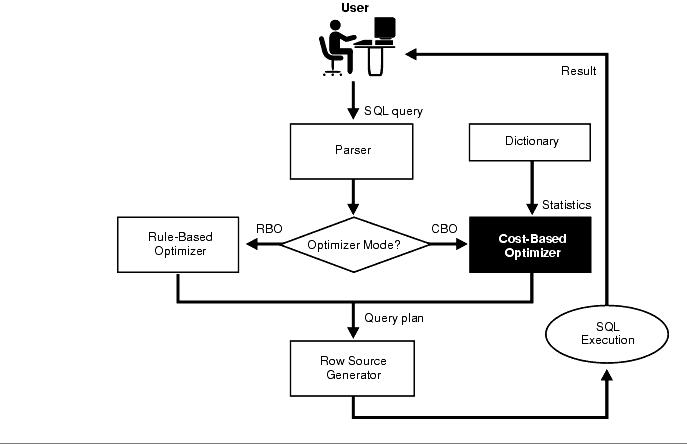
\includegraphics[width=\textwidth]{03_Related_Work/OracleArchitecture.png}
  \caption{Oracle Architecture \cite{Oracle2004Basics}}
  \label{OracleArchitecture}
\end{figure}



Die Oracle Architektur zur Verarbeitung von Anfragen \cite{Oracle2004Basics} (vgl. Abb. \ref{OracleArchitecture})  beginnt wie die meisten Systeme mit einer SQL Anfrage, die von einem Parser in eine Interne Repräsentation gebracht wird. Der Parser übernimmt dabei zwei Funktionen. Auf der einen Seite die Syntaktische Analyse. Es wird geprüft, ob die SQL Anfrage die korrekte Syntax besitzt. Auf der anderen Seite eine Semantische Analyse. Diese prüft beispielsweise ob Datenbank Objekte und Objekt-Attribute  korrekt referenziert werden. Nachdem diese beiden Schritte ausgeführt wurden unterscheidet der Optimierer ob ein \ac{RBO} oder ein \ac{CBO} zum Einsatz kommt. Mit Version 11g der Oracle Datenbank wird der \ac{RBO} nicht mehr unterstützt und ausschließlich auf den \ac{CBO} gesetzt \cite{dba_oracle2015}.

Der \ac{QO} führt bei der Verarbeitung die folgenden drei Schritte aus:

\begin{itemize}
\item Eine Menge potentieller Pläne wird basierend der SQL Anfrage selbst und Hinweisen, die durch den Nutzer eingegeben werden, generiert.
\item Der Optimierer schätzt die Kosten für jeden Plan basierend auf Kosteninformationen über die Anfrage und Storage Charakteristiken der Tabellen, Indexe und Partitionen, die durch ein Statement zugegriffen werden können.

Die Kostenschätzung für den Zugriff auf entsprechende Datensätze und die Reihenfolge der Joins wird nach ihrem Verbrauch von Ressourcen wie I/O, CPU und Memory geschätzt.

Pläne mit höheren Kosten benötigen mehr Zeit zur Ausführung als Pläne mit niedrigeren Kosten. Falls Pläne parallel ausgeführt werden können, ist die Ressourcen Nutzung nicht direkt abhängig von der verwendeten Zeit.

\item Der Optimierer vergleicht die Kosten der Pläne und wählt den kostengünstigsten Plan aus.
\end{itemize}

Das Ergebnis des Optimizers ist ein Plan, der zum Ausführen der Anfrage geeignet ist und als kostenoptimal eingeschätzt wird.


\subsection{Kostenbasierte Transformation in Oracle}

Traditionelle Relationale Datenbank Systeme führen, wie bereits dargestellt, die Transformation von Anfragen in zwei Phasen durch: Logische und physische Phase. In der logischen Phase wird die gegebene Anfrage zuerst durch einen Rewriter angewendet, hier kommen Heueristiken oder Regeln zum Einsatz. Der traditionelle pyhsische Optimizer arbeitet mit einem einzelnen Query Block aus Restriktionen über Tabellen, Projektionen und Joins. Die Physische Optimizerungsphase befasst sich mit Access Methoden, Join Orders und join Methoden die genutzt werden, um effiziente Pläne zu erzeugen.

Query Transformation werden entweder als Rewriter Systeme oder als Extention des Plan generators mit dem pyhsichen Optimierer implementiert. Der erste Ansatz skaliert nicht in komplexen kommerziellen Systemen, der zweite Ansatz ist nur einfach auf ein paar wenige Transformationen anzuwenden. 
Bisher wurden zuerst Rewriter Rules angewendet und dann die Nutzung von Cost Based Trasnformations angewendet. \cite{ahmed2006cost} argumentiert, dass einige Heueristiken nicht immer ein optimales Ergebnis erzeugen und daher mit Hilfe von Cost Based Methoden geprüft werden sollten, bevor sie auf eine Anfrage angewendet werden.


Oracle hat die kostenbasierte Transformation, die logische Transformation und die physische Optimierung kombiniert, um den optimalen Execution Plan zu finden. Der Logische Teil des Systems teilt sich in Heueristiken und kostenbasierte Transformationen. Die kostenbasierten Trasnformatioenen funktionieren wie folgt:

\begin{itemize}
\item Transformationsalorithmen konvertieren gesamte under teil Anfrage Bäume in sequentiell gleiche Form
\item Stae Spaces für verschiedene Transformationen
\item State Space Search Algorithmen
\item Möglichkeit zur Deep Copy von Anfrage Böcken und Ihrer Consitutues
\item Cost estimation techique (physical optimizer)
Transformation derective und cost annotations
\end{itemize}

Unterschiedliche Transformationsregeln werden auf unterschiedliche Teile der Anfrage angewendet. So kann beispielsweise die Entschachtelung nur auf verschachtelte Elemente der Anfrage angewendet werden. 

Die Bäume werden Bottom up transformiert während der Optimierung. Verschiedene Alternativen für eine oder mehrere Transformationen für Elemente in einem Query Tree generieren unterschiedliche States innerhalb des Ste Space of Transformation. Eine Deep kopy wird gemacht bevor ein bestimmter status erreicht wird und dessen Kosten durch den Aufruf des physischen Optimierers geschätzt werden. Die Evaluation von jedem States. Der Transformationsstage, der die besten Kosten bietet wird zurück auf den Ursprungstree angewendet.

Die Oracle Transformationen werden immer hintereinander angewendet. Eine Transformatiosnregel wird immer auf den ganzen Baum angewendet, erst danach folgt die nächste Regel. Die Reihenfolge ist diese: Common sub expression factorization, JPS view merging, join elimination, subquery unnesting, group by distinct view merging, group pruning, predicate move around, set operator factorization, disjunction into union-all exansion, star transfomration and join predicate pushdown. Von dieser Reihenfolge kann jedoch in bestimmten Fällen abgewichen werden. 



\subsubsection{State Space Search Techniques}
Bei der Suche nach einem Plan mit Hilfe von kostenbasierender Transformation stellt sich die grundsätzliche Frage nach einem Trade-off zwischen optimalen Kosten und Execution Kosten. Die Suche nach einer Transformation lohnt sich nur dann, wenn die Kosten für die Suche nach einer besseren Transformation gemeinsam mit der Ausführung der eigentlichen Anfrage geringer ist als die bisher gefundenen Pläne.

Die Frage nach diesem Problem stellt sich insbesondere, wenn eine große Menge an möglichen alternativen Plänen bestehen.. Existieren viele einzelne Objekte einer Anfrage, seien es Query Blocks, Tables join edges predikate, gibt es auch die Möglichkeit, dass viele Regeln auf die Objekte angewendet und somit viele alternative Pläne erzeugt werden können. Wenn $N$ Objekte vorhanden sind und auf diese $N$ Objekte eine Transformation $T$ angewendet wird, dann werden nur durch diese eine transformation $2^N$ verschiedene Pläne generiert. Dies Menge wächst weiter, wenn mehrere Transformationen auf die bestehenden Objekte angewendet werden können. 


Um dieses kombinatorische Problem der vielen oin permutationen zu lösen wurden mehrere randomizierte Algorithmen vorgeschlagen. Tabu Search, Genetic Search, Iterative Improvement...

chst mit der Anzahl der Trasnfromationsobjekte. Wenn die Anzahl der Transformationsobjekte klein ist, dann ist eine enumerative Transformationstechnik mit Hilfe Exhaustive search des States vielleicht machbar. Da aber die Anzahl der möglichen Optimierungen mit der Zeit steigt, müssen andere Techniken angewendet werden:

\begin{itemize}
\item 
\end{itemize}

\subsubsection{Subquery Entschachtelung}

\subsubsection{Join Elimination}

\subsubsection{Filter Predicate Move Around}

\subsubsection{Group Pruning}


\section{Pellenkoft Rulsets}

Bei der Erforschung eines Search Spaces kommen in regelbasierten \ac{QO} Transformationsregeln zum Einsatz. Pellenkoft et al. \cite{pellenkoft1997duplicate} \cite{manegold2000multi} \cite{pellenkoft1997complexity} stellt drei Regelsets zur Verfügung, die bei der Erzeugung eines Search Spaces zum Einsatz kommen können.



Zu Beginn besteht ein Search Space aus einem Plan. Dieser Plan stellt die Eingabe dar. Auf ihn werden Transformationsregeln angewendet. Neue Pläne entstehen. Sollten diese Pläne noch nicht vorhanden sein, werden sie dem Suchraum hinzugefügt. Pläne auf die bereits alle anwendbaren Transformationsregeln angewendet wurden, werden als besuchte Pläne bezeichnet. Sobald alle Pläne besucht wurden und somit auf alle Pläne Transformationsregeln auf alle Pläne angewendet wurden, ist der Suchraum vollständig erforscht und keine weiteren Pläne können gefunden werden. Der Actual Search Space ist ausgeschöpft.

Mehrere Transformationsregeln werden gemeinsam als Regelsets bezeichnet. Pellenkoft et al. unterscheidet zwischen Regelsets, die Pläne mehrfach generieren können und Regelsets, die duplikatfrei sind. Beispielsweise kann durch die Anwendung der Regel Kommutativität auf einen Plan und erneute Anwendung auf dessen Resultat  der ursprüngliche Plan generiert werden. Im Folgenden werden zwei Regelsets vorgestellt, die Duplikate bilden und ein Regelset, das duplikatsfrei ist.


\subsection{Regelset mit Duplikaten}

Eines der Regelsets, das zur Erzeugung eines Bushy Tree Space genutzt werden kann, ist $RS-B0$. Es besteht aus drei Regeln:

\begin{itemize}
\item Kommutativität: $$ A \Join B \to B \Join A$$
\item Rechte Assoziativität: $$(A \Join B) \Join C \to A \Join (B \Join C) $$
\item Linke Assoziativität: $$A \Join (B \Join C) \to (A \Join B) \Join C$$
\end{itemize}

Das Regelset ist redundant, da mit Hilfe von Kommutativität und rechter Assoziativität linke Assoziatvität (und vis-à-vis) erzeugt werden kann. Möchte man die Redundanz vermeiden, lässt sich Regelset $RS-B1$ erstellen. Es basiert auf Kommutativität und einer Swap genannten Regel:

\begin{itemize}
\item Swap $$ (A \Join B) \Join C \to (A \Join C) \Join B $$
\item Bottom Commutativitity $$ B_1 \Join B_2 \to B_2 \Join B_1$$
\end{itemize}


<<<<<<< HEAD
Durch die Anwendung der Regeln aus $RS-B0$ und $RS-B1$ können Pläne doppelt erzeugt werden. Am einfachsten ist dies an Hand von Kommutativität zu zeigen. Wird auf den Plan $a \Join b$ Kommutativität angewendet, entsteht b JOIN a, dann entsteht durch  die erneute Anwendung von Kommutativität auf den neuen Plan B JOIN A wieder der ursprüngliche Plan.

Ebenfalls können sich bei komplexeren Plänen     Teilpläne gleichen. Beispielsweise enthält der Plan $(A \Join B) \Join C$ den gleichen Subplan wie $C \Join (A \Join B)$. Um solche Duplikate zu verhindern, wird von Pellenkoft das Prinzip der Äquivalenzklasse angewendet.
=======
Ebenfalls können sich bei komplexeren Plänen     Teilpläne gleichen. Beispielsweise enthält der Plan $(A \JOIN B) \JOIN C$ den gleichen Subplan wie $C \JOIN (A \JOIN B)$. Um solche Duplikate zu verhindern, wird von Pellenkoft das Prinzip der Äquivalenzklasse angewendet.
>>>>>>> 2dbe3382d95b975a93a2c2789dd91dda3468d5cc



\subsection{Duplikatfreie Regelsets}
Durch die Anwendung on $RS_B0$ bzw. $RS_B1$ ist es möglich, dass Varianten des Plans erneut erzeugt werden. Dieser Gefahr trägt das Regelset RS-B2 Rechnung. Es sieht vor, dass eine Regel nur genau einmal ausgeführt und andere Regeln nur einmal pro Operator ausgeführt werden dürfen. Dieses Regelset besteht aus:


\begin{itemize}
\item Kommutativität: $$ A \Join B \to B \Join A$$
\item Rechte Assoziativität: $$(A \Join B) \Join C \to A \Join (B \Join C) $$
\item Linke Assoziativität: $$A \Join (B \Join C) \to (A \Join B) \Join C$$

\item Exchange $$(A \Join B) \Join (C \Join D) \to (A \Join D) \Join (C \Join B) $$
\end{itemize}



\subsubsection{Kreuzproduktfreie Regelsets und Vollständigkeit}

Die bisherigen Regelsets können zu Kreuzprodukten führen. Ebenfalls ist nicht geklärt, ob die Regelsets vollständig sind und alle möglichen kreuzproduktfreien Bäume erzeugen. Im Folgenden wird zuerst der Begriff der Kreuzproduktfreiheit eingeführt und basierend auf diesem Begriff die Vollständigkeit erläutert.

Ein Kreuzprodukt kann bei den vorliegenden Plänen dann entstehen, wenn durch die Anwendung einer Regel ein Join zwischen zwei Relationen gebildet wird, die zuvor keine Kante auf einem gegeben Join Tree hatten.

Eine Technik um Kreuzproduktfreiheit bei den bisherigen Regelsets herzustellen, ist die Unterdrückung von Kreuzprodukten die auch als \ac{CPS} bezeichnet wird. Der Ansatz funktioniert so, dass eine Regel, falls sie ein Kreuzprodukt erzeugt zwar als ausgeführt markiert, jedoch nicht der Baum in den Search Space aufgenommen wird. Somit werden Kreuzprodukte zwar erzeugt, aber nicht in den Suchrraum aufgenommen. Regelsets, die diese Art von Kreuzproduktunterdrückung anwenden, erhalten das Suffix CPS. Somit entstehen aus den Regelsets RS-B0, RS-B1 und RS-B2 die Regelsets RS-B0-CPS, RS-B1-CPS und RS-B2-CPS.


Eine andere wichtige Eigenschaft von Regelsets ist Vollständigkeit. Sie setzt voraus, dass Kreuzproduktfreiheit gegeben ist. Vollständigkeit liegt dann vor, wenn alle kreuzproduktfreien Pläne in einem Suchraum erzeugt wurden.


<<<<<<< HEAD
=======
\subsubsection{Unvollständigkeit von RS-02}


\begin{figure}[h]
  \centering
  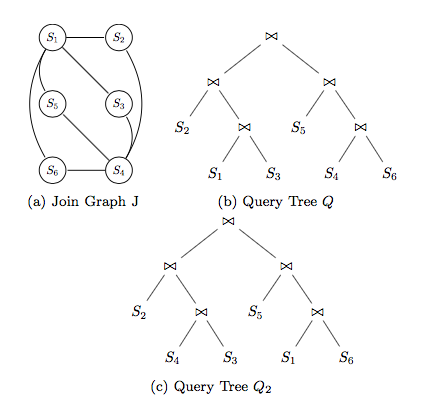
\includegraphics[width=\textwidth]{03_Related_Work/Incompleteness_RS-B2-CPS.png}
  \caption{Incompletness of RS-B2-CPS}
  \label{Incompleteness_RS-B2-CPS}
\end{figure}


\cite{shanbhag2014optimizing} stellt fest, dass RS-B0-CPS und RS-B1-CPS vollständig sind. Die Vollständigkeit von RS-B2-CPS wird jedoch in Frage gestellt und die Unvollständigkeit mit Hilfe eines Beispiels belegt. Als Beispiel dient eine Menge von Relationen, die mit Hilfe des Jointrees J (\ref{fig:Incompleteness_RS-B2-CPS}) miteinander gejoint sind. Der Initale Anfragebaum $Q1$ ist in \ref{fig:Incompleteness_RS-B2-CPS} dargestellt. Das gewünschte Ergebnis nach einer Transformation $Q2$  findet sich in \ref{fig:Incompleteness_RS-B2-CPS}. 

Bei RS-B2-CPS dürfen die Regeln R2, R3, R4 nur jeweils einmal auf einen Join-Operator angewendet werden. Keine der Regeln darf danach auf den neu generierten Operator angewendet werden. Die In \ref{fig:Q1} und \ref{fig:Q2} zeichnet sich dadurch aus, dass die Relationen $R1$ und $R4$ vertauscht sind.







\subsubsection{Vorschlag von RS-Graph}

\subsection{JOIN SETS}

Basierend auf dem bisherigen Wissen, wurden durch X und y einige neue Begriffe festgelegt:W
Ein Base Equivalence Knoten in einem expandierten LQDAG ist ein Äquivalenzknoten, der keinen Join Operator als Kinder hat. Ein solcher Knoten kann entweder eine Relation sein oder darf keine Join Operatoren als Kinder beinhalten.

Ein Join Tree ist in einem expandierten LQDAG ein Baum in der LQDAG dessen Wurzel ein Äuqivalenzknoten und jeder interne Knoten entweder ein Äquivalenzknoten oder ein Join Operator und jeder untergeordneter Knoten ein Äuqivalenzknoten ist.

Der Maximale JOIN Tree ist in einem expandierten LQDAG ein Join Tree, bei dem jeder Leaf knoten ein Base Equivalence Node ist.

Ein Join-Set für einen Äquivalenzknoten E ist in einem expandierten LQDAG ein Paar $J = (S, P)$ bei dem S ein Set von Äquivalenzknoten ist, deren 

\subsection{Ruleset RS-Graph}
Neben den bereits etablierten Regeln wird eine neue Regel für den Volcano Optimizer von \cite{shanbhag2014optimizing} vorgestellt. Die neue Transformationsregel $RS-Graph$ ersetzt die bisherigen Regeln und die bisherigen Regelsets. Die neue Regel erzeugt basierend auf einem Planknoten direkt alle möglichen äquivalenten Pläne. Somit sind alle Pläne unter einem bestimmten Äquivalenzknoten mit der Anwendung nur einer Regel erzeugt.

Die Regel $RS-Graph$ verwendet dazu die Subroutine $GraphRule$. Sie wird auf den Join Tree angewendet, falls die beiden mit einem Operator verbundenen Knoten A und B und deren Mitterknoten $P$. Für jedes Paar der J $$equivalence nodes A,B and parent equivalence node P. For each pair of join-set (jsA,jsB) ∈ A.JoinSets∗B.JoinSets, we merge the pair to form a join-set js. We define the merge of the two join-sets jsA = (V1,P1) and jsB = (V2,P2) as (V1∪V2,P1 ∧P2).$$

Um wiederholte Berechnungen des selben Join TRees zu vermeiden wird zudem geprüft, ob der Eltern-Äquivalenzknoten bereits $js$ beinhaltet. $$To check if two join- sets at an equivalence node are equal, it is sufficient to check if they have same equivalence nodes. If the join-sets have the same equivalence nodes, then they will also have the same predicates.$$

Für alle Join Sets $js$ des Parent nodes werden daraufhin zuerst alle JOIN partitionen gebildet bei denen $S_1 \Join S_2$ mit 

Sollte der $js$ noch nicht existieren, wird dieser dem JOIN Set hinzugefügt. Ein Graph wird basierend auf den $js$ gebildet, der mit Hilfe der Methode Partition in alle Partitionen getrennt wird. Aus denen wiederum Bäume erstellt werden, die an das Resultat zurückgegeben werden.

Die SubRoutine Create Graph, gibt ein JOIN Set, das JS einen Join Graphen aus, der




\subsection{Discussion}
Die Implementierung der neuen Regel wurde in einem Java basierten regelbasierten Optimierer implementiert. Dieser Optimierer “ProtoJ” ist eine Übersetzung des Optimierers Proto aus C++ in Java. Für die Implementierung mussten neue Felder den Äquivalenzklassen hinzugefügt werden.

Die Generierung der Resultate find ohne Pruning statt und kosten für die Kostenberechnung wurden nicht einbezogen. Ebenfalls bleiben Regeln bestehen, die für denn SELECT Pushdown verantwortlich sind, als teil der Normalisierungsphase. 

Es wurden sowohl Star, Chain als auch Clique Queries getestet. Die Experimente fanden auf einem Intel i5 3.5 GHz mit 8 GB Ram statt. Es wurde festgestellt, dass die Geschwindigkeit der Optimierung verbessert werden konnte, dadurch, dass die Optimierung mehrfach durchgeführt wurde. Dieses Verhalten wurde auf Javas JIT Kompilierungsstrategie zurückgeführt. Die erst den Code Kompiliert, wenn er auch tatsächlich gebraucht wird. Um sicherzustellen, dass der Kompilierte Code nicht wieder während der Ausführung vergessen geht mussten spezielle Flags für die JVM gesetzt werden. Das Ergebnis war, dass die Dauer zwar verglichen zu den schnellsten Test ohne das Flag langsamer, aber dafür konstant blieben.

Ebenfalls wurde bei Ruleset $RS_B1$ geprüft, ob der gesamte Search Space erreicht wurde, indem die Anzahl der Äquivalenten Knoten und Operatoren im LQDAG gezählt wurden. Diese Zahl wurde mit der Zahl der Knoten in RS-Graph verglichen. Da beide zahlen gleich war, wird davon ausgegangen, dass beide Regelsets das selbe Ergebnis erzeugen. Eine Prüfung, die dies belegt fand aus technischen Gründen nicht statt.






ersetzten X und Y die bisher gezeigten Regeln des Volcano Optimizers mit einer neuen Transformationsregel: RS-Graph. Die Regel kommt zur Anwendung, falls ein Graph dem Pattern $E_1 \Join E_2$ entspricht. Ist dies der Fall wird die Funktion $GraphRule(\Join, E_1, E_2, parent)$ aufgerufen. Sie erzeugt ein Set von allen Join Operatoren unter dem Equivalenzklasse des $parent$-Knotens.




\subsubsection{}



\subsection{Patition zu Graph}



Die Methode Partition gibt eine Menge von Partitionen zurück. Jede Partition bezeichnet eine Menge von Knoten. Sowohl $S_1$ als auch $G\\S_1$ sind Teil dieser Menge, falls beide zwischen beiden im Joni-Graphen miteinander verbunden sind. Im Gegensatz zu anderen Regeln, die pro Anwendung der Regel nur immer einen neuen Knoten zurückgegeben haben, gibt die neue Regel immer Bäume zurück, die alle möglichen Join Operatoren unterhalb des ROOT Operators beinhalten.
>>>>>>> 2dbe3382d95b975a93a2c2789dd91dda3468d5cc

\section{GraphRule und Unvollständigkeit von RS-B2}

Die von Pellenkoft et al. entwickelten Regelsets, dienen als Grundlage für regelbasierte Optimierer wie Volcano. \cite{shanbhag2014optimizing} untersuchten die Vollständigkeit der vorgestellten Regel und fügten den bestehenden Regelsets ein neues hinzu, das alle andere Regelsets zum Join Reordering obsolet macht und zudem eine erheblich bessere Performance liefert.

Die Untersuchungen \cite{shanbhag2014optimizing} wurden mit dem Optimierer PyroJ durchgeführt. PyroJ ist ein Optimierer, der basierend auf Pyro \cite{roy2001multi} erstellt wurde und dem Volcano Optimizer nachempfunden ist. Zuerst wurden die Regelsets auf ihre Vollständigkeit hin geprüft. Neben der Prüfung auf Vollständigkeit konnte auch die neue Regel GraphRule implementiert und so bzgl. ihrer Performance getestet werden.



\subsection{Implementierung von PyroJ}

PyroJ basiert auf dem von \cite{roy2001multi} in C++ Implementierten Optimierer Pyro und wurde automatisch von C++ nach Java übersetzt. Der Optimierer Pyro wurde nach dem Vorbild des Volcano Optimierers entwickelt. Volcano wurde als Vorbild gewählt, da es sich bei Volcano um einen hoch-respektierten, state-of-the-art, regelbasierten Optimierer handelt, der auch die Basis von kommerziellen Datenbanksytemen wie MS SQL Server ist. Außerdem ist Volcano, wie zuvor besprochen, hoch erweiterbar: Das Datenmodell, Executionmodell ist leicht erweiterbar, Transformationsregeln und Operatoren lassen sich hinzufügen. 

Einer der Unterschiede zwischen Volcano und Pyro ist die Trennung zwischen logical / physical Plan Generierung und der Suche nach dem optimalen Plan. Im Gegensatz zu Volcano werden erst alle logische Pläne für einen \ac{LQDAG} generiert, daraufhin werden alle Pläne in physische Pläne umgesetzt und basierend auf diesen Plänen der günstigste Plan ausgewählt.

Der Volcano Optimizer hingegen berechnet zuerst einen logischen Plan und generiert für diesen Plan dann alle physischen Pläne. Für diese Pläne wird der günstigste Plan gesucht. Die anderen Pläne müssen nicht mehr im Speicher vorgehalten werden. Daraufhin kann dann der nächste logische Plan generiert werden und die Kosten des günstigsten Plans mit dem bisher günstigsten Plan verglichen werden. Der Vorteil dieses Verfahrens ist, dass gerade bei großen Search Spaces der Plan im Speicher gehalten werden kann und suboptimale Pläne nicht länger als nötig gespeichert werden.

Genau wie das Volcano Projekt wird eine Memofunktion verwendet. \cite{roy2001multi} weist daraufhin, dass diese Memofunktion erst später dem Volcano Optimizer hinzugefügt wurde. Dadurch war es beispielsweise möglich, dass bei einer Anfrage, die aus $(A \Join B \Join C) \cup (B \Join C \Join D)$ zwei Äquivalenzknoten für den Knoten $B \Join C$ gebildet werden, obwohl alle Teilpläne von $A \Join B$ immer äquivalent sein werden und somit kein Grund besteht, die Pläne mehrfach zu berechnen. Pyro verwendet eine Memodatenstruktur, um die mehrfache Generierung des selben Teilplans zu unterbinden.

Ein weiterer Unterschied zu Volcano ist, dass es  bei Pyro kein Optimizer generiert wird, sondern der Optimizer von vornherein in C++ geschrieben ist. Eine Übersetzung aus einem Description\-File hin zu C\-Code findet daher nicht statt.

\subsection{Getestete Regeln und Regelsets}

\cite{shanbhag2014optimizing} und \cite{roy2001multi} geben an, dass sie die Regelsets \textit{RS-B0}, \textit{RS-B1} und \textit{RS-B2} implementieren. Im Gegensatz zu Pellenkoft wird im Regelset \textit{RS-B1} nicht die Regel Swap verwendet, sondern Left\-Associtativity (vgl. \ref{PellenkoftVsPyro}). Beide Regeln sind jedoch semantisch ähnlich genug und können mit Hilfe von Kommutativität in einander überführt werden. Ebenfalls ist eine genaue Unterscheidung der Reihenfolge der Anwendung, ähnlich wie bei Volcano nicht möglich. Alle Regeln laufen immer in einer vorgegeben Reihenfolge ab.

\begin{table}[ht]
\begin{tabular}{|l|l|l|}
\cline{1-3}
{\bf Regelmenge} & {\bf Pellenkoft}                                                                                                  & {\bf Pyro(J)}                                                                                                       \\ \cline{1-3}
{\bf RS-B0}   & \begin{tabular}[c]{@{}l@{}}Left Associativity\\ Right Associativity\\ Commutativity\end{tabular}            & \begin{tabular}[c]{@{}l@{}}Left Associativity\\ Right Associativity\\ Commutativity\end{tabular}              \\ \cline{1-3}
{\bf RS-B1 }  & \begin{tabular}[c]{@{}l@{}}Swap\\ Bottom Commutativity\end{tabular}                                         & \begin{tabular}[c]{@{}l@{}}Left Associativity\\ Commutativity\end{tabular}                                    \\ \cline{1-3}
{\bf RS-B2 }  & \begin{tabular}[c]{@{}l@{}}Left Associativity\\ Right Associativity\\ Commutativity\\ Exchange\end{tabular} & \begin{tabular}[c]{@{}l@{}}Left Associativity\\ Right Associativity\\ Commutativity\\ Exchange\end{tabular}   \\ \cline{1-3}
\end{tabular}
\caption{Unterschiede zwischen Pellenkoft und Pyro(J)}
\label{PellenkoftVsPyro}
\end{table}




\subsection{Unvollständigkeit von \textit{RS-B2}}



\begin{figure}[ht]
  \centering
  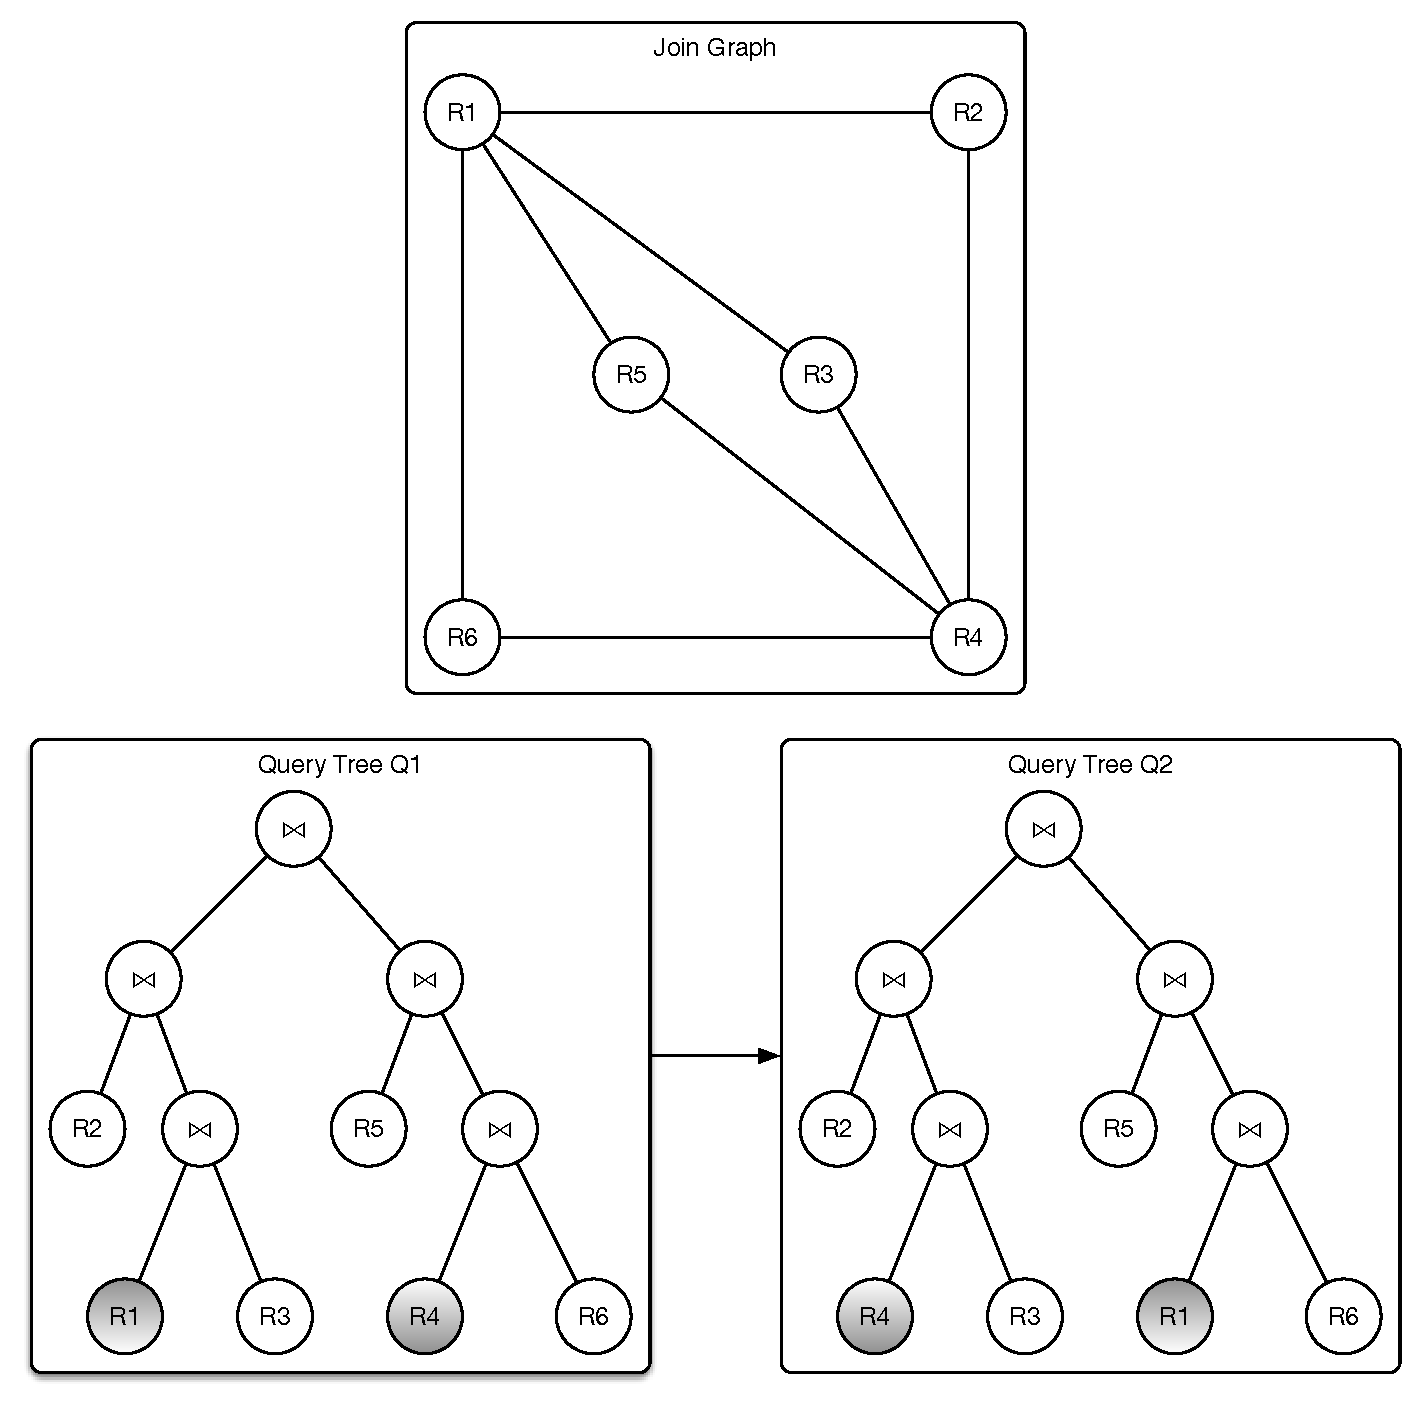
\includegraphics[width=\textwidth]{02_Related_Work/Graphs.pdf}
  \caption{Incompletness of RS-B2-CPS}
  \label{Incompleteness_RS-B2-CPS}
\end{figure}


Die Unvollständigkeit von \textit{RS-B2} wurde auf zwei Arten gezeigt. Auf der einen Seite wurde an Hand des Beispiel \ref{Incompleteness_RS} gezeigt. Im konkreten Beispiel sollte \textit{R1} und \textit{R4} getauscht werden, wobei das Regelset \textit{RS-B2} zum Einsatz kommen sollte. Anhand des gegebenen Join Graphen ist die Transformation zwar Teil des Suchraums, kann jedoch durch die Regeln nicht erreicht werden. Das Regelset ist daher unvollständig.

Ebenfalls wurden unterschiedliche Abfragen mit Hilfe des Optimierers optimiert und dahingehend geprüft, ob die selbe Menge an Plänen aus den unterschiedlichen Regelsets entstehen kann. Wie erwartent war die Menge der Pläne, die aus \textit{RS-B0} nur \textit{RS-B1} entstanden sind gleich, die Menge der \textit{RS-B2} Pläne stark reduziert. (vgl. \ref{tabelle)}.

Da nicht alle Pläne gefunden werden konnten, liegt es nahe, dass der optimale Plan möglicherweise nicht Teil des erforschten Suchraums ist. \cite{shanbhag2014optimizing} stellen fest, dass das Ergebnis mit \textit{RS-B2} erzeugt wurde bzgl. der berechneten Kosten um den Faktor 1.86 schlechter war, als die Pläne, die mit Hilfe eines vollständigen Regelsets erzeugt wurden. Wie genau die Zahl 1.86 zustande gekommen ist, ist nicht genauer begründet.

Es lässt sich also feststellen, dass mit Hilfe des Regelsets \textit{RS-B2} weniger Pläne im Suchraum gefunden werden konnten, als mit Hilfe des Regelsets \textit{RS-B1} bzw. \textit{RS-B2}. Außerdem wurde festgestellt, dass Pläne aus unvollständigen Regelsets nicht immer den optimalen Plan beinhalten.





\subsection{Unvollständigkeit von RS\-02}




\cite{shanbhag2014optimizing} stellt fest, dass RS-B0-CPS und RS-B1-CPS vollständig sind. Die Vollständigkeit von RS-B2-CPS wird jedoch in Frage gestellt und die Unvollständigkeit mit Hilfe eines Beispiels belegt. Als Beispiel dient eine Menge von Relationen, die mit Hilfe des Jointrees J (\ref{fig:Incompleteness_RS-B2-CPS}) miteinander gejoint sind. Der Initale Anfragebaum \textit{Q1} ist in \ref{fig:Incompleteness_RS-B2-CPS} dargestellt. Das gewünschte Ergebnis nach einer Transformation \textit{Q2}  findet sich in \ref{fig:Incompleteness_RS-B2-CPS}. 

Bei \textit{RS-B2-CPS} dürfen die Regeln \textit{R2}, \textit{R3}, \textit{R4} nur jeweils einmal auf einen Join-Operator angewendet werden. Keine der Regeln darf danach auf den neu generierten Operator angewendet werden. Die In \ref{fig:Q1} und \ref{fig:Q2} zeichnet sich dadurch aus, dass die Relationen \textit{R1} und \textit{R4} vertauscht sind.


Die Vollständigkeit wurde auch mit Hilfe des PyroJ Optimierers geprüft. Hierbei wurde an Hand von Star-Queries  die Unvollständigkeit belegt. Wie in Abb. \ref{CompletenessResults} zu sehen, wurden mit Hilfe von \textit{RS-B2} nur knapp die Hälfte aller äquivalenten Pläne gefunden. Ebenfalls wird betont, dass die geschätzten Kosten des besten Plans, der durch \textit{RS-B2} erzeugt wurde um den Faktor 1.86 im Vergleich zu \textit{RS-B1} niedrigere geschätzte Kosten hatte.







\subsection{Vorschlag von RS-Graph}

\subsection{JOIN SETS}

Basierend auf dem bisherigen Wissen, wurden durch X und Y einige neue Begriffe festgelegt: W.
Ein Base Equivalenz Knoten in einem expandierten LQDAG ist ein Äquivalenzknoten, der keinen Join Operator als Kinder hat. Ein solcher Knoten kann entweder eine Relation sein oder darf keine Join Operatoren als Kinder beinhalten.

Ein Join Tree ist in einem expandierten LQDAG ein Baum in der LQDAG dessen Wurzel ein Äuqivalenzknoten und jeder interne Knoten entweder ein Äquivalenzknoten oder ein Join Operator und jeder untergeordneter Knoten ein Äuqivalenzknoten ist.

Der Maximale JOIN Tree ist in einem expandierten LQDAG ein Join Tree, bei dem jeder Leaf Knoten ein Base Equivalence Node ist.

Ein Join-Set für einen Äquivalenzknoten E ist in einem expandierten LQDAG ein Paar $J = (S, P)$ bei dem S ein Set von Äquivalenzknoten ist, deren 

\subsection{Regelmenge RS-Graph}
Neben den bereits etablierten Regeln wird eine neue Regel für den Volcano Optimizer von \cite{shanbhag2014optimizing} vorgestellt. Die neue Transformationsregel \emph{RS-Graph} ersetzt die bisherigen Regeln und die bisherigen Regelsets. Die neue Regel erzeugt basierend auf einem Planknoten direkt alle möglichen äquivalenten Pläne. Somit sind alle Pläne unter einem bestimmten Äquivalenzknoten mit der Anwendung nur einer Regel erzeugt.

Die Regel \emph{RS-Graph} verwendet dazu die Subroutine $GraphRule$. Sie wird auf den Join Tree angewendet, falls die beiden mit einem Operator verbundenen Knoten A und B und deren Mitterknoten $P$. Für jedes Paar der J %\emph{equivalence nodes A,B and parent equivalence node P. For each pair of join-set (jsA,jsB) ∈ A.JoinSets∗B.JoinSets, we merge the pair to form a join-set js. We define the merge of the two join-sets jsA = (V1,P1) and jsB = (V2,P2) as (V1∪V2,P1 ∧P2).}

Um wiederholte Berechnungen des selben Join Trees zu vermeiden wird zudem geprüft, ob der Eltern-Äquivalenzknoten bereits $js$ beinhaltet. $$To check if two join- sets at an equivalence node are equal, it is sufficient to check if they have same equivalence nodes. If the join-sets have the same equivalence nodes, then they will also have the same predicates.$$

Für alle Join Sets $js$ des Parent nodes werden daraufhin zuerst alle JOIN partitionen gebildet bei denen $S_1 \Join S_2$ mit 

Sollte der $js$ noch nicht existieren, wird dieser dem JOIN Set hinzugefügt. Ein Graph wird basierend auf den $js$ gebildet, der mit Hilfe der Methode Partition in alle Partitionen getrennt wird. Aus denen werden wiederum Bäume erstellt, die an das Resultat zurückgegeben werden.

Die SubRoutine Create Graph, gibt ein JOIN Set, das JS einen Join Graphen aus, der




\subsection{Diskussion}
Die Implementierung der neuen Regel wurde in einem Java basierten regelbasierten Op den Äquivalenzklassen neue Felder hinzugefügt werden.

Die Generierung der Resultate findet ohne Pruning statt und Kosten für die Kostenberechnung werden nicht einbezogen. Ebenfalls bleiben Regeln bestehen, die für denn SELECT Pushdown verantwortlich sind, als Teil der Normalisierungsphase. 

Es wurden sowohl Star, Chain als auch Clique Queries getestet. Die Experimente fanden auf einem Intel i5 3.5 GHz mit 8 GB Ram statt. Es wurde festgestellt, dass die Geschwindigkeit der Optimierung verbessert werden konnte, dadurch, dass die Optimierung mehrfach durchgeführt wurde. Dieses Verhalten wurde auf Javas JIT Kompilierungsstrategie zurückgeführt, die erst den Code kompiliert, wenn er auch tatsächlich gebraucht wird. Um sicherzustellen, dass der Kompilierte Code nicht wieder während der Ausführung vergessen wird, mussten spezielle Flags für die JVM gesetzt werden. Das Ergebnis war, dass die Dauer zwar verglichen zu den schnellsten Tests ohne das Flag langsamer, aber dafür konstant blieb.

Ebenfalls wurde bei Regelmenge $RS_B1$ geprüft, ob der gesamte Search Space erreicht wurde, indem die Anzahl der Äquivalenten Knoten und Operatoren im LQDAG gezählt wurden. Diese Zahl wurde mit der Zahl der Knoten in RS-Graph verglichen. Da beide Zahlen gleich waren, wird davon ausgegangen, dass beide Regelsets das selbe Ergebnis erzeugen. Eine Prüfung, die dies belegt fand aus technischen Gründen nicht statt.






Ersetzten X und Y die bisher gezeigten Regeln des Volcano Optimierers mit einer neuen Transformationsregel: RS-Graph. Die Regel kommt zur Anwendung, falls ein Graph dem Pattern $E_1 \Join E_2$ entspricht. Ist dies der Fall wird die Funktion $GraphRule(\Join, E_1, E_2, parent)$ aufgerufen. Sie erzeugt ein Set von allen Join Operatoren unter dem Äquivalenzklasse des $parent$-Knotens.







\subsection{Partition zu Graph}



Die Methode Partition gibt eine Menge von Partitionen zurück. Jede Partition bezeichnet eine Menge von Knoten. Sowohl $S_1$ als auch $G\\S_1$ sind Teil dieser Menge, falls beide zwischen beiden im Join-Graphen miteinander verbunden sind. Im Gegensatz zu anderen Regeln, die pro Anwendung der Regel nur immer einen neuen Knoten zurückgegeben haben, gibt die neue Regel immer Bäume zurück, die alle möglichen Join Operatoren unterhalb des ROOT Operators beinhalten.





Das bestehende Regel-Framework von Volcano wurde von \cite{shanbhag2014optimizing} mit einem neuen Regelset und einer neuen Regel erweitert. Das neue Regelset Graph Rule soll alle bestehenden Regeln zur JOIN-Tree Enumeration ersetzen. Im Gegensatz zu den vergleichsweise ineffektiven Regelsets, die bisher bekannt waren, setzt die neue Regel auf state-of-the-art, kreuzproduktfreie Join-Enumeratoren zur Suche nach äquivalenten Plänen. Damit kombiniert die neue Regel die Vorteile eines hoch erweiterbaren Systems wie Volcano mit der Geschwindigkeit von neuartigen Join-Enumeratoren.

Die neue Regel gibt nicht nur eine neue Variante des Query-Trees zurück, sondern bestimmt gleich auf einmal alle äquivalenten Pläne. Die Erweiterbarkeit des Volcano-Optimierers ermöglicht es auch eine solche komplexe, neue Regel zu implementieren.

Die neue Regel wird in drei Schritten umgesetzt. Zuerst werden die Subtrees bestimmt, auf die ein Paritionierungsalgorithmus im nächsten Schritt angewendet werden kann. Mit Hilfe der einzelnen Partitionen werden dann neue Bäume aufgebaut, die als alternative Pläne zurückgegeben werden. Diese drei Schritte sind auch in Abb. \ref{GraphRule} zu sehen.

\subsection{Routinen}





Um die Funktion der neuen Regel im Detail zu beschreiben, führt \cite{shanbhag2014optimizing} eine Reihe neuer Begriffe für einen Baum ein:

\begin{itemize}
\item \textit{Base Equivalence Node}: dieser Knoten bezeichnet einen Äuqivalenzknoten, der keine JOIN-Operatoren als dessen Kinder besitzt.
\item \textit{Join Equivalence Node}: dieser Begriff bezeichnet einen Äquivalenzknoten, der mindestens eine JOIN Operation untergeordnet hat.
\item \textit{Maximal Join Tree}: Dieser Baum ist ein Baum, der entweder Äquivalenzknoten oder einen JOIN Operator untergeordnet hat.
\item Ein \textit{Maximal join Tree} ist ein Baum, dessen Kinder immer EuqivalenceNodes sind.
\item Ein \textit{Join Set} für einen Äquivalenzknoten E ist ein Paar $J = (V, P)$ bei dem $V$ ein Set von Äquivalenknoten ist und deren Kinder seine 
\end{itemize}


\subsection{Implementierung}
Die Implementierung des neuen Regelsets wurde auf Basis des Query Optimierers PyroJ vorgenommen. PyroJ ist eine Übersetzung des in C++ entwickelten Optimierers Pyro, der an der Universität Bombay entwickelt wurde und das Volcano-Framework implementiert.

Alle Tests wurden auf einem Computer mit Intels Core i5 3.5 GHz mit 8 Gbyte Arbeitsspeicher und Ubuntu 11.10 durchgeführt. Die genaue Java Version und Einstellungen der JVM sind (fast) vollständig unbekannt.

Wie von \cite{shanbhag2014optimizing} beschrieben, wurde während er Performance Test festgestellt,dass sich die Dauer für die Ausführung einer Optimierung stark unterscheidet.Für die Durchführung einer Optimierung wurden zu Beginn erheblich höhere Werte festgestellt. Gerade die ersten Anfragen hatten eine besonders hohe Laufzeit. Erklärt wurde dieses Verhalten durch den Java \ac{JIT}-Compiler. Ebenfalls wurde erkannt, dass der Java eigene Code Optimierer HotSpot die Ergebnisse verfälschen kann. 

Während der Performance Tests wurde festgestellt, dass sich.........


\subsection{Probleme auf Grund der Plattformwahl}
Die Implementierung der neuen Regel wurde auf Basis von PyroJ vorgenommen. PyroJ ist eine Übersetzung des von ITT Bombay entwickelten Systems Pyro, das eine Implementierung des Volcano-Frameworks ist. PyroJ, das in Java implementiert ist, entstand durch eine automatische Konvertierung des C++ Codes von Pyro. 

Die Implementierung der Experimente wurde auf Basis von PyroJ vorgenommen. PyroJ ist eine Übersetzung des in C++ geschriebenen Query Optimierers Pyro nach Java. Der Optimierer wurde an der IIT Bombay gebaut und ist eine Implementierung des Volcano Optimization Frameworks.

Die Experimente wurden auf einem Intel Core i5 3.5 GHz Computer mit 8 Gbyte Arbeitsspeicher und Ubuntu 11.10 vorgenommen. Es wurde festegestellt, dass die Implementierung des Codes in Java verglichen zu C++ einigen Overhead generiert, der die Laufzeit der Optimierung negativ beeinflusst. Ebenfalls wurde festgestellt, dass die Laufzeit zur Optimierung einer Anfrage erheblichen Schwankungen unterlegen ist. Insbesondere konnten stark unterschiedliche Laufzeiten bei den selben Queries festgestellt werden. Queries, die zu Beginn ausgeführt wurden, wurden langsamer ausgeführt. Dieses Phänomen wurde auf den Java JIT-Compiler (HotSpot) zurückgeführt. Dieser kompiliert nur die zur Ausführung notwendigen Teile des Programms und führt Optimierungen zur Laufzeit durch. Um konstante Laufzeiten für die selbe Anfrage zu erzielen, wurde nach eigenen Angaben die JIT-Kompilierung ausgeschaltet. Außerdem wurde das Java HotSpot JVM flag $-XX:CompileThreshold=1$ gesetzt und einige große Queries ein paar mal optimiert, um sicherzustellen, dass alle Funktionen auch kompiliert werden bevor sie ausgeführt werden.
 

\subsection{Kritik} \todo{Wo soll dieser Teil eigentlich hin? Evaulation/ Related Work / Implementierung}


Die Implementierung des Frameworks wirft einige Fragen auf. Auf der einen Seite wird durch den Autor selbst festgestellt, dass durch die Wahl einer anderen Code Basis (C++ statt Java) Ergebnisse mit weniger Overhead erzielt werden könnten. Warum also die Entscheidung zur Implementierung in Java gefallen ist, bleibt unbeantwortet.

Auch die Probleme, die durch den JIT Compiler entstanden sind, sind außergewöhnlich. Zuerst wurde die Kompilierung nach eigenen Angaben abgeschaltet und dann wiederum sichergestellt, dass alles kompiliert wurde, indem große Anfragen optimiert wurden. Was genau mit dieser Aussage gemeint ist bleibt unbeantwortet.  Ich nehme an, dass nur das JVM Flag $-XX:CompileThreshold=1$ gesetzt wurde. Dieses Flag gibt an, nach wie vielen Methodenaufrufen ein Stück Java Code in Maschinencode kompiliert wird. Der Standardwert liegt bei 10000 \cite{oracle2015VMOptions}. Dank dieses Flags wird bereits beim ersten Aufruf einer Methode die Methode auch kompiliert. Warum dieser Umweg gewählt wurde, bleibt wage.

Ein weiterer Grund für Fehler bei der Messung kann die Wahl der Plattform im Allgemeinen sein. Da die Ausführung des Programms zu jedem beliebigen Zeitpunkt durch die Garbage Collection unterbrochen werden kann, können Messungen der Laufzeit nur schwer vorgenommen werden. Um wenigstens einen Hinweis auf diese Messfehler zu finden, wäre eine Nutzung der JVM Flags $ -verbose:gc -XX:+PrintGCDateStamps -XX:+PrintGCDetails$ möglich gewesen. Diese Flags geben an, wann die Garbage Collection zuschlägt und wieviel Zeit diese zur Ausführung benötgt. \cite{andreasson2015JVM}  


Warum also trotz all dieser möglichen Fehlerquellen und Ungenauigkeiten gerade Java zum Einsatz gekommen ist, ist unklar und wenig verständlich. Insbesondere da eine Alternative in C++ mit Pyro bereitstand.




